% npj Artificial Intelligence Article, using the official Springer Nature
% December 2024 sn-nature template. Figures are generated by
% r2\_decoder\_sparse\_readout\_audit/scripts/50_make_manuscript_figures.py.

\documentclass[pdflatex,sn-nature]{sn-jnl}

\usepackage{graphicx}
\usepackage{amsmath,amssymb,amsfonts}
\usepackage{booktabs}
\usepackage{array}
\usepackage{seqsplit}
\usepackage{url}

\raggedbottom
\newcommand{\hashvalue}[1]{\texttt{\seqsplit{#1}}}

\begin{document}

\title[Auditing cross-model sparse readouts in protein language models]{Auditing semantic and causal claims from cross-model sparse readouts in protein language models}

\author*[1]{\fnm{Zipeng} \sur{Liu}}\email{liuzipeng@tju.edu.cn}
\author[1]{\fnm{Coauthors} \sur{to be added}}

\affil*[1]{\orgdiv{Affiliation to be updated}, \orgname{Institution to be updated}, \orgaddress{\city{City}, \country{Country}}}

\abstract{Mechanistic interpretability often treats recurring sparse features as evidence of shared concepts, although recurrence does not establish semantic validity or causal control. We audited this inference in three generative protein language models using cross-layer transcoders. A fixed 200-sequence procedure identified 38 feature triplets at $|r|\geq0.90$, versus at most one under 30 pair/layer-specific reassignments; a separate 500-sequence cohort yielded eight triplets with no exact identity overlap. Exploratory analyses associated 37 triplets with local sequence, protein position or transcoder-input norm, and three with initiator-methionine positions and high unnormalized received attention. Specified pretrained-model interventions failed their gates. A prospectively frozen synthetic calibration with a fixed planted comparator passed in three model seeds, with sensitivity, specificity and false-discovery rate of 1, 1 and 0 and effect-recovery ratio approximately 1; this establishes pipeline sensitivity only at the planted effect size, not pretrained-model causality. A steering pilot showed no positive evidence but contained a feature-sign selection defect. Sparse-readout recurrence was cohort and procedure sensitive and requires independent semantic and causal validation before supporting biological or design claims.}

\maketitle

Recurring components across model fits or architectures are often treated as especially persuasive explanations. Reproducibility, however, answers a different question from semantic validity or causal relevance. Recent work in explainable artificial intelligence distinguishes faithful participation in a prediction from human-aligned meaning, shows that biological interpretations can inherit training and architecture biases, and argues that explanation methods require use-case-specific correctness criteria and prospective controls \cite{lee2025selfexplanation,esserskala2023reliable,haufe2026formalization,pesapane2026evidence}. Component-level methods such as Concept Relevance Propagation and SemanticLens make latent concepts searchable or attribution-linked, but their semantic accessibility does not by itself establish behavioral use \cite{achtibat2023crp,dreyer2025semanticlens}. A feature can therefore be stable, nameable and predictive while remaining unsuitable as a scientific concept or intervention target.

Protein language models (PLMs) provide a consequential test domain for this distinction. ProtGPT2, ZymCTRL, ProGen and ProGen2 showed that autoregressive or conditionally prompted models can sample protein-like sequences, enzymes and family-conditioned designs from large sequence corpora \cite{ferruz2022protgpt2,munsamy2022zymctrl,madani2023large,nijkamp2023progen2}. Masked PLMs established that self-supervised sequence training can encode structural, functional and evolutionary information \cite{rives2021biological,elnaggar2022prottrans,rao2021structure,lin2023esm}. Contemporary work stresses family-aware evaluation, representation uncertainty, explicit control constraints and experimental validation rather than treating correlated computational scores as function \cite{alwer2026kinform,dumontet2026enzyme,prabakaran2026uncertainty,zhu2026controllable,watson2023rfdiffusion}. Evo~2 further couples sparse-feature exploration to a fully released genomic model and experimentally tested guided designs \cite{brixi2026evo2}. These capabilities make explanations attractive for model evaluation and design, but the biological stakes increase the cost of conflating an internal correlate with a mechanistic handle.

Sparse-autoencoder studies of ESM-2 and related encoders report features associated with Gene Ontology terms, protein families, binding sites and motifs \cite{gujral2025proteinSAE,adams2025mechanisticBiology,simon2025interplm}. Work on superposition, sparse dictionaries, transcoders and crosscoders similarly aims to expose variables or computational graphs hidden in dense activations \cite{elhage2022toy,bricken2023monosemanticity,cunningham2024sparse,templeton2024scaling,dunefsky2024transcoders,ameisen2025circuit,lindsey2024crosscoders}. A recent synthesis connects identifiability, sparse recovery and behavioral assessment, underscoring that a recovered code still needs task-grounded validation \cite{klindt2026unifying}. Yet probing work has repeatedly shown that decodability is not evidence that a variable is used by a model, motivating counterfactual tests and ablations \cite{hewitt2019control,elazar2021amnesic,meng2022rome,wang2023ioi}. Sparse internal patterns can support causal localization in some language-model settings \cite{wu2025sparsepatterns}, but the evidential link must be tested rather than inferred.

Here we audit sparse-readout recurrence across ProtGPT2, ZymCTRL and ProGen2-medium. We propose four estimands for a prospective benchmark: recurrence under a frozen cross-model procedure ($R$), biological association remaining after low-level covariates ($S$), effects of faithful interventions beyond matched controls ($C$), and prospectively validated downstream utility ($U$). This four-estimand benchmark was not executed end to end in the present study; the historical analyses provide bounded evidence for only parts of it, and a prospectively frozen planted benchmark calibrates only synthetic intervention sensitivity. We also compare linear probes on the tensors used as transcoder inputs with probes on the corresponding sparse codes. The proposed framework is deliberately diagnostic. The historical audit identifies procedure-specific cross-model recurrence and an N-terminal subset, while exposing limitations in the original annotation gate, the steering score, the activation-space terminology and the exploratory wider-dictionary test. Figure~\ref{fig:workflow} summarizes the independent data and gates that a future execution would require for each estimand.

\begin{figure}[t]
\centering
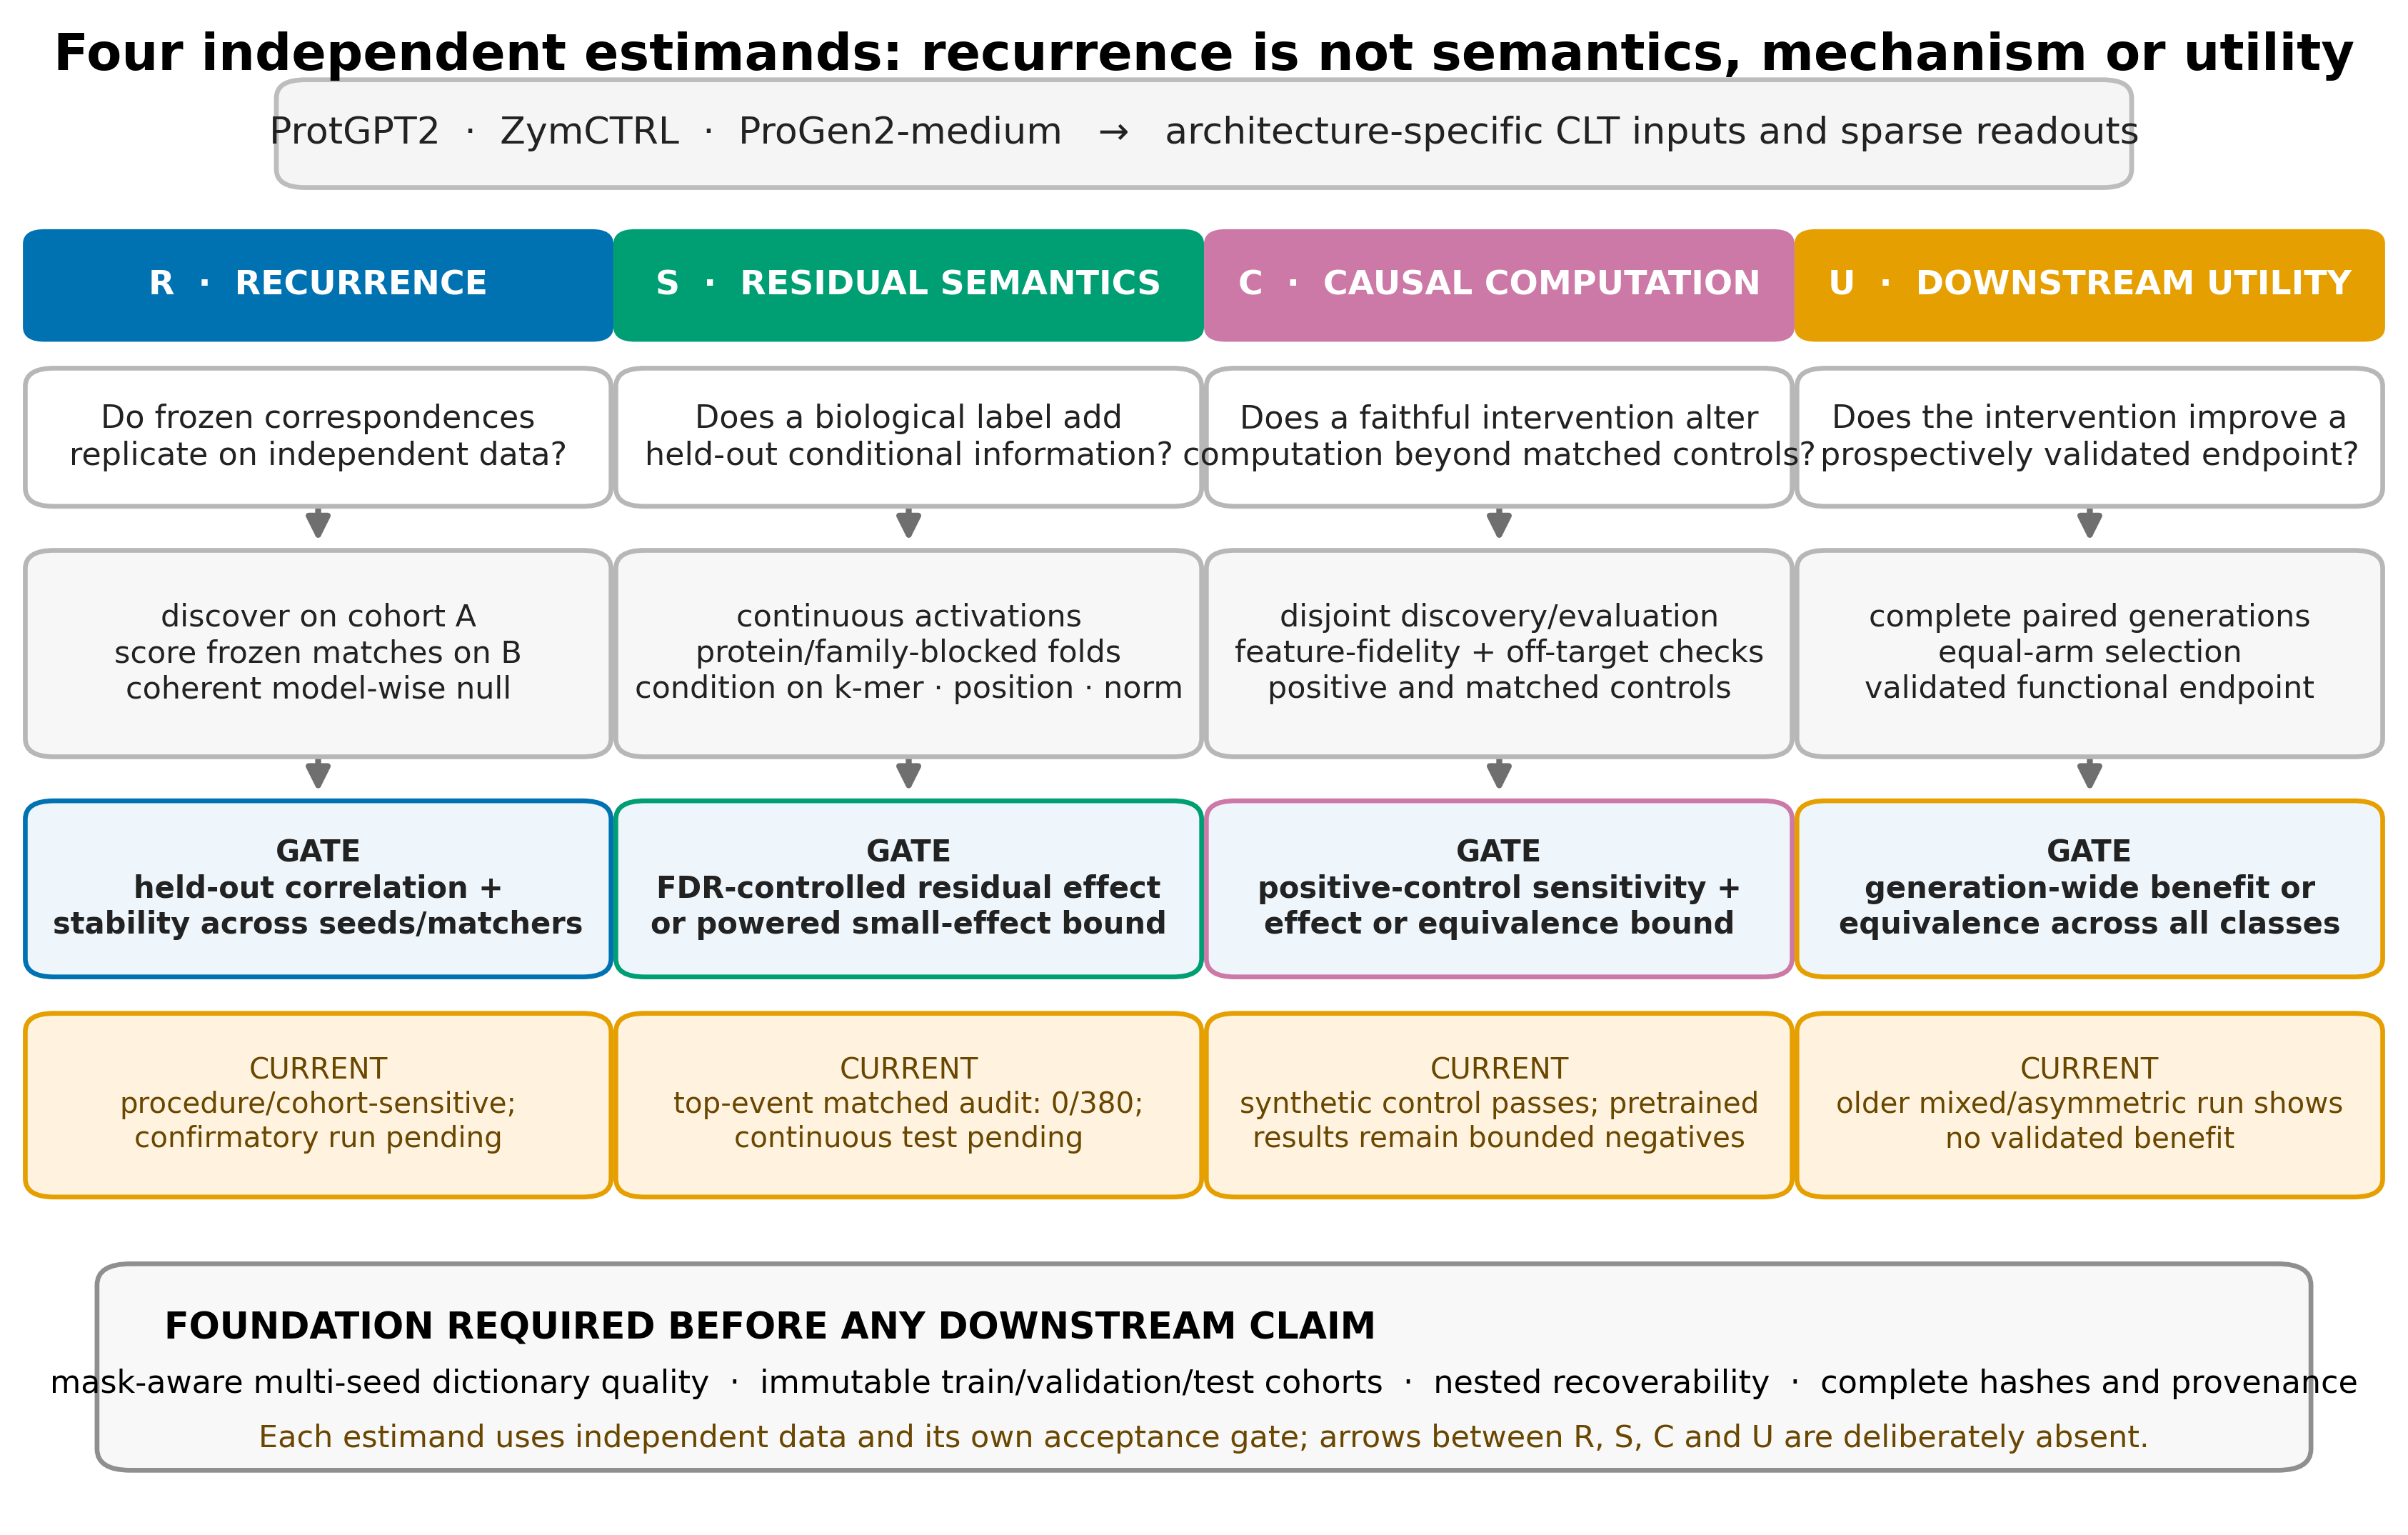
\includegraphics[width=\textwidth]{figures/figure_01_workflow.pdf}
\caption{\textbf{Audit workflow for cross-model sparse readouts.}
The proposed prospective audit separates recurrence ($R$), residual semantics ($S$), causal computation ($C$) and downstream utility ($U$). Each estimand would have independent data, controls and an acceptance gate; none would be inferred from a preceding column. The complete R/S/C/U benchmark was not executed in this study; only a synthetic planted-control sensitivity subgate was completed prospectively. Mask-aware multi-seed dictionaries, immutable cohorts, nested recoverability and complete provenance form the proposed shared foundation. Orange boxes distinguish the bounded historical evidence from outstanding confirmatory work.}
\label{fig:workflow}
\end{figure}

\section{Results}\label{sec:results}

\subsection{A fixed cross-model matching procedure identifies recurrent readouts}

We first asked whether independently trained protein generators contain sparse readouts with matched activation profiles. The analysis used ProtGPT2, ZymCTRL and ProGen2-medium. For each model we trained a sparse dictionary as a cross-layer transcoder (CLT), using it as a readout over transformer computations rather than as a standalone predictor. The ProtGPT2 and ZymCTRL reference dictionaries spanned 36 layers, with width $d_\mathrm{CLT}=8192$, TopK sparsity $k=128$ and 200{,}000 training steps; the ProGen2-medium atlas checkpoint covered 27 layers with $d_\mathrm{CLT}=4096$ and $k=64$ (Supplementary Table~1). The reported atlas used one reference dictionary per model and was not replicated across dictionary seeds. Quick-evaluation reconstruction and dead-feature statistics were uneven and included padded positions, so we treat them as unmasked diagnostics rather than definitive dictionary-quality estimates.

On a fixed balanced cohort of 200 sequences, we matched feature activation profiles at three anchor depths and retained exact three-model triplets when all pairwise matches exceeded an absolute-correlation threshold. Within this procedure, the atlas contained 38 triplets at $|r|\geq0.90$, 30 at $|r|\geq0.95$ and eight at $|r|\geq0.98$ (Fig.~\ref{fig:atlas}a and Supplementary Table~2). Because matching used $|r|$, anticorrelated profiles counted as recurrent even though they can represent complementary rather than equivalent behaviour; signed and positive-only replication is outstanding. A 30-replicate pair/layer-specific sequence-reassignment null produced a mean of 0.07 triplets and a maximum of one at $|r|\geq0.90$. Each model-pair/layer edge used a separate reassignment, so null triangles were not generated by one coherent model-wise permutation. A separate 500-sequence UniRef50 cohort yielded eight triplets at 0.90 and three at 0.95, with no exact feature-identity overlap with the canonical 38. The canonical comparison therefore documents cohort- and procedure-specific recurrence relative to the implemented null; it does not estimate conservation across arbitrary cohorts, layers or matching algorithms.

The original Swiss-Prot annotation gate could not support its intended conclusion. It binarized the top 100 of 122{,}671 residue positions, whose event entropy was 0.00661 nats, and compared mutual information with an unattainable 0.1-nat threshold. We therefore removed that gate. In an exploratory reanalysis of the saved top events, 224 of 380 triplet--label associations met Benjamini--Hochberg-adjusted $q<0.05$ under a global position null, whereas 0 of 380 met that threshold under a within-protein null matched on amino-acid identity and position. Failure to meet this exploratory gate does not prove absence of biological alignment because only selected top events were retained and the analysis was designed after the gate audit. Separately, a 38-dimensional triplet basis did not match 2,560-dimensional ESM-2 mean-pooled embeddings on Pfam-family, Enzyme Commission (EC) top-class or secondary-structure-fraction probes (Supplementary Table~3); that dimension-unmatched comparison is a representation diagnostic, not a semantic null.

\begin{figure}[t]
\centering
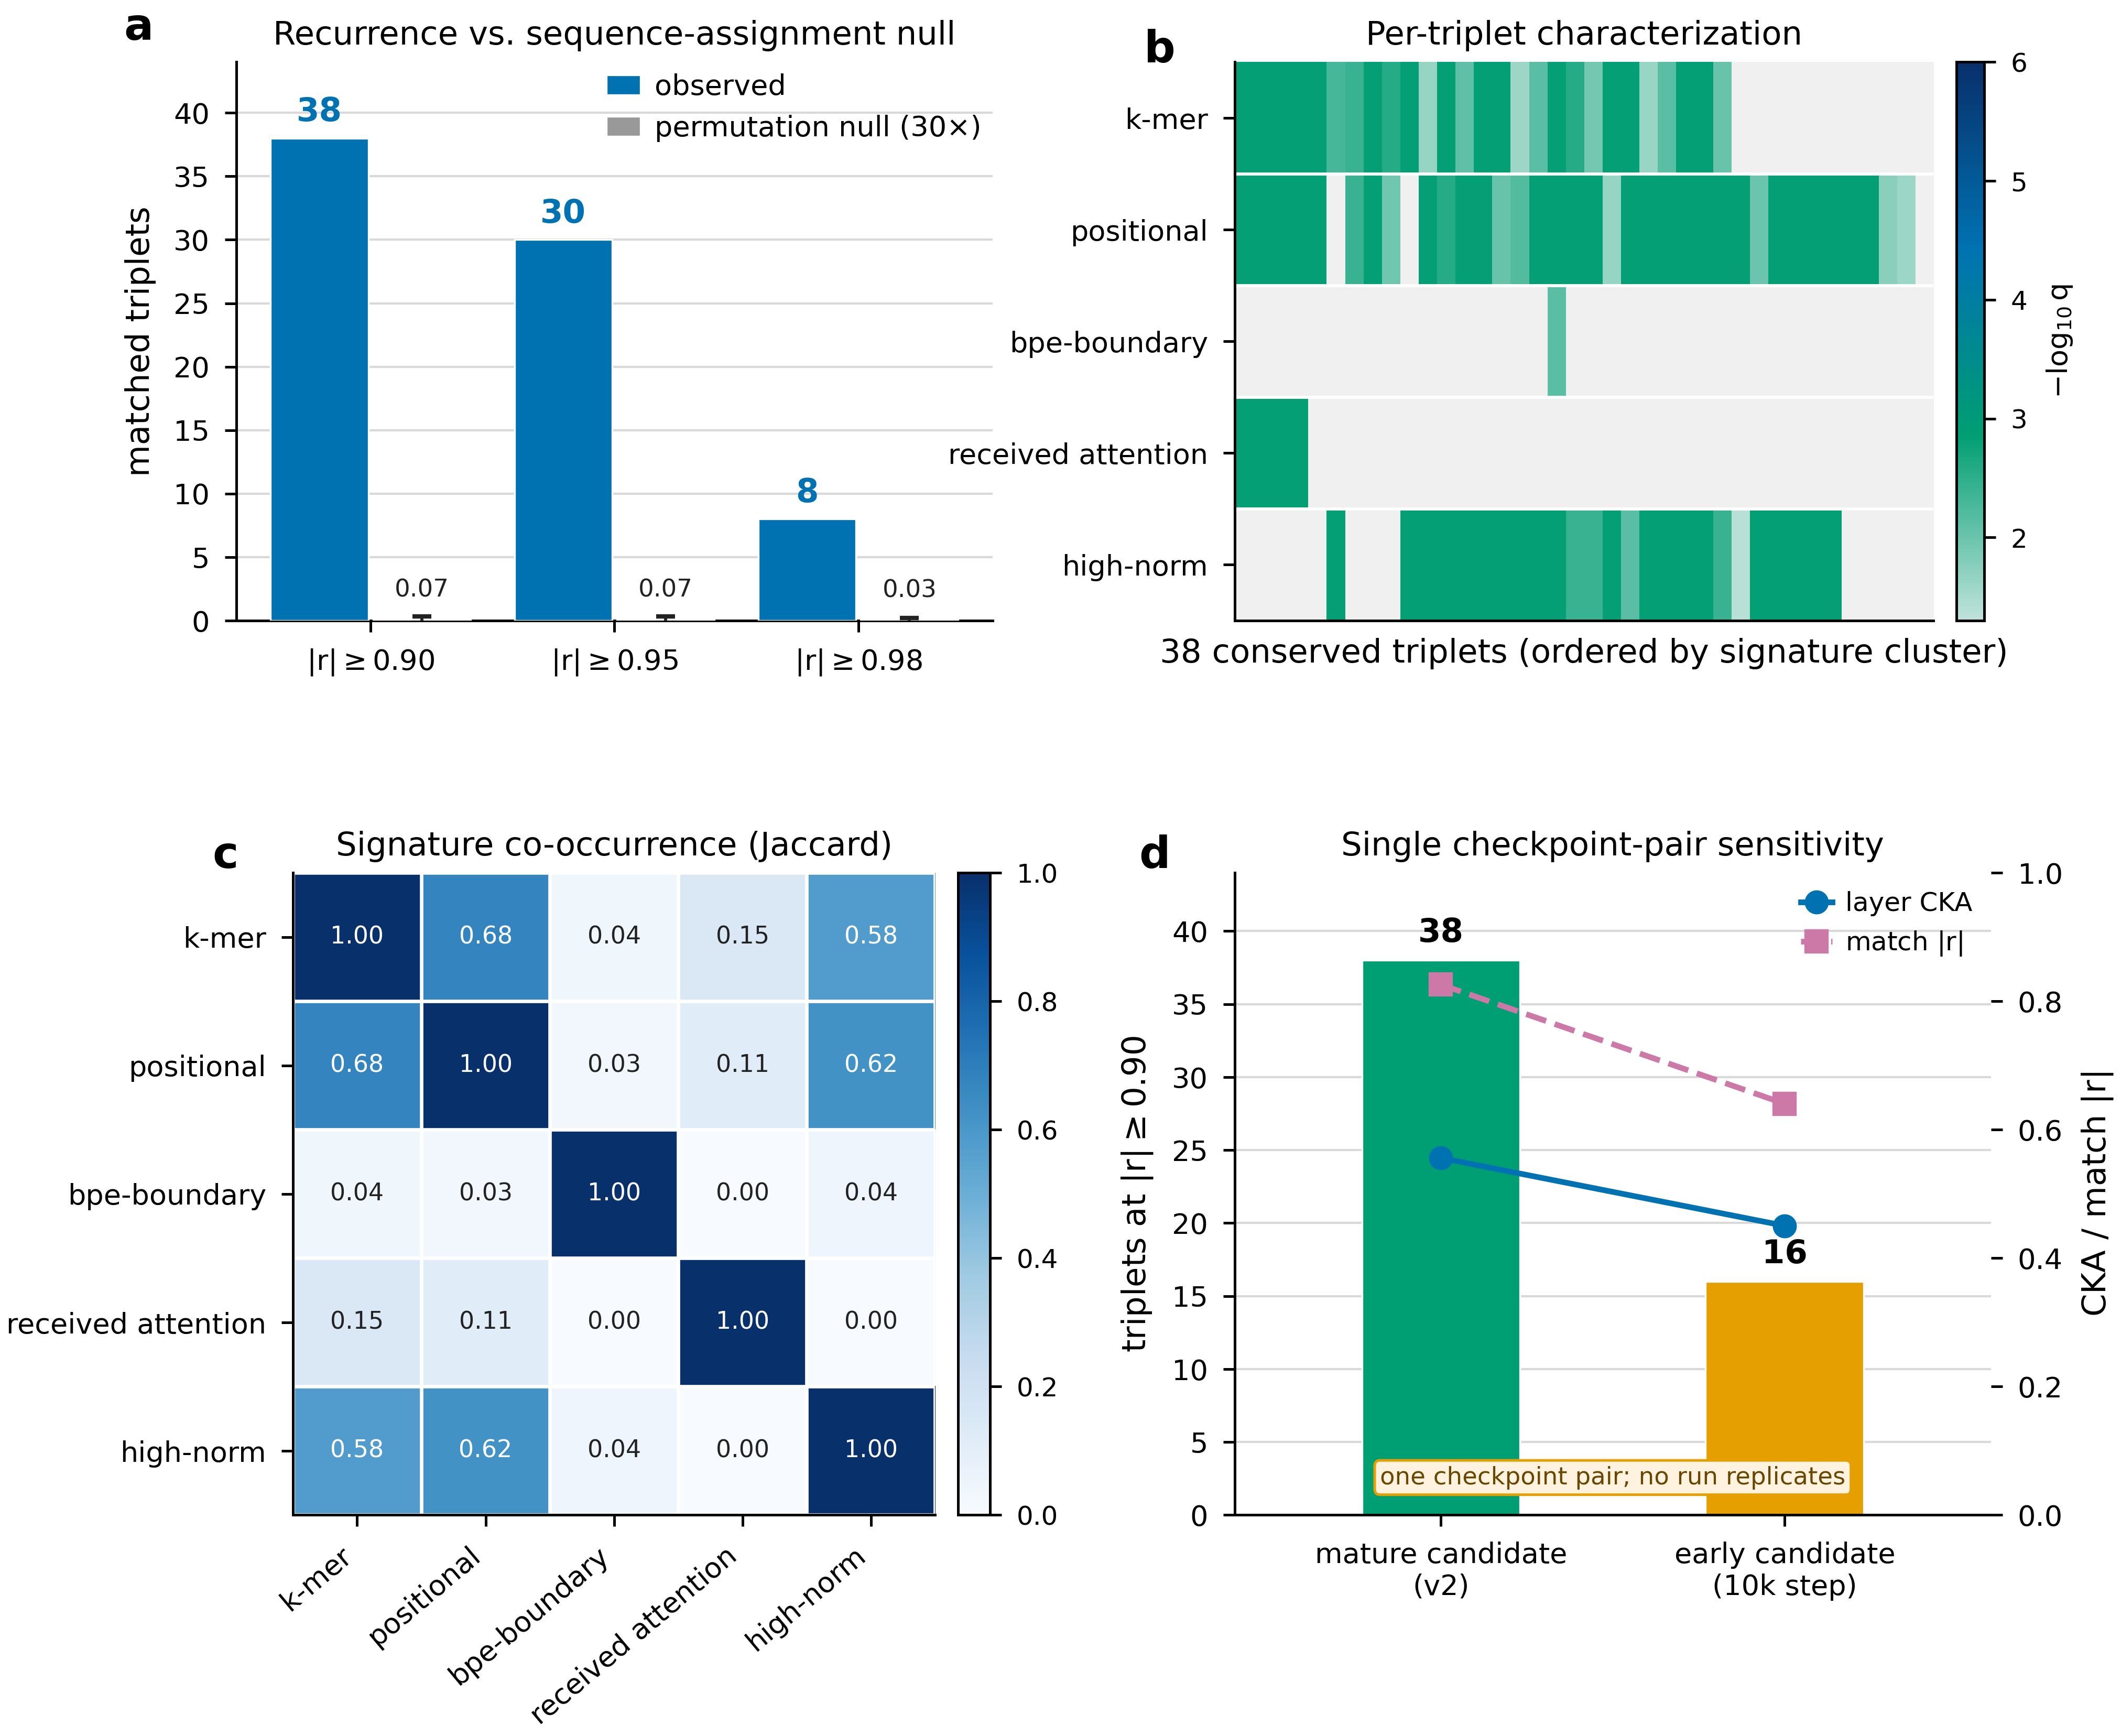
\includegraphics[width=\textwidth]{figures/figure_02_sparse_readout_atlas.pdf}
\caption{\textbf{Cross-model sparse-readout recurrence and exploratory characterization.}
\textbf{a}, Exact three-model triplet counts at three absolute-correlation thresholds compared with 30 pair/layer-specific sequence reassignments (error bars, s.d.); these are not coherent model-wise permutations. \textbf{b}, Exploratory characterization heatmap for the 38 triplets across five low-level tests. Shading denotes Benjamini--Hochberg-adjusted $q<0.05$ under the implemented residue-level permutation procedures; these tests do not fully account for within-protein dependence. ``High norm'' refers to the architecture-specific CLT input tensor. \textbf{c}, Jaccard overlap among triplet sets detected by the five low-level association tests, not overlap across cohorts or matching algorithms. \textbf{d}, A single mature-versus-early checkpoint-pair comparison; the result motivates checkpoint sensitivity as a candidate diagnostic but does not validate it across seeds or training trajectories. A separate UniRef50 cohort recovered fewer triplets and no canonical feature identities; that sensitivity is reported in the text and Supplementary Table~2.}
\label{fig:atlas}
\end{figure}

\subsection{Recurrent triplets show overlapping low-level associations}

We next characterized the triplets without assigning biological names. The implemented tests covered k-mer enrichment, normalized protein position, ProtGPT2 BPE-boundary enrichment, same-layer received-attention correlation and CLT-input norm correlation. Thirty-seven of 38 triplets were detected on at least one test after Benjamini--Hochberg correction, and 21 were detected on three or more (Fig.~\ref{fig:atlas}b and Supplementary Table~4). Positional, k-mer and high-norm associations occurred in 35, 27 and 25 triplets, respectively. Because residue positions within a protein were not treated as independent experimental units in every null and the stronger of the 3-mer and 5-mer results was selected, these counts are exploratory association summaries rather than confirmatory biological categories.

The detected associations were not mutually exclusive. k-mer and position overlapped in 25 triplets (Jaccard 0.676), position and CLT-input norm in 23 (Jaccard 0.622), and k-mer and CLT-input norm in 19 (Jaccard 0.576; Fig.~\ref{fig:atlas}c). The most defensible description is therefore that the recurrent readouts covary with several low-level properties; the analysis does not identify which property, if any, is represented independently.

The mature reference checkpoint pair recovered 38 triplets at $|r|\geq0.90$, whereas an early 10k-step pair recovered 16; mean layer centred kernel alignment \cite{kornblith2019similarity} and mean matched-feature correlation were also higher (Fig.~\ref{fig:atlas}d and Supplementary Table~5). This single comparison shows sensitivity to training stage and motivates recurrent-triplet count as a candidate development diagnostic. Validation requires additional checkpoints, seeds and held-out cohorts.

\subsection{N-terminal readouts coincide with high unnormalized received attention}

T011, T018 and T023 formed a clear N-terminal subset in the saved top-firing rows (Fig.~\ref{fig:sink}). For each triplet, all 100 rows came from the first two residues of 100 unique proteins, and their contexts were dominated by initiator-methionine motifs (Supplementary Table~6). Their correlations with same-layer received attention were 0.921, 0.914 and 0.885. However, received attention was averaged over queries without normalizing for the greater causal opportunity of early key positions, and the residue-event enrichment tests did not use protein as the statistical unit. We therefore describe these triplets as N-terminal readouts with high unnormalized received attention, not as established attention-sink features. T025 provided a non-N-terminal comparator, firing on HNC/NHI/IHN-like contexts.

The robust observation is positional and sequence-based: three recurrent readouts concentrate at protein starts. Whether their attention correlation exceeds a position-conditioned causal baseline remains open, and none of the intervention results below shows that these features implement or control an attention sink.

\begin{figure}[t]
\centering
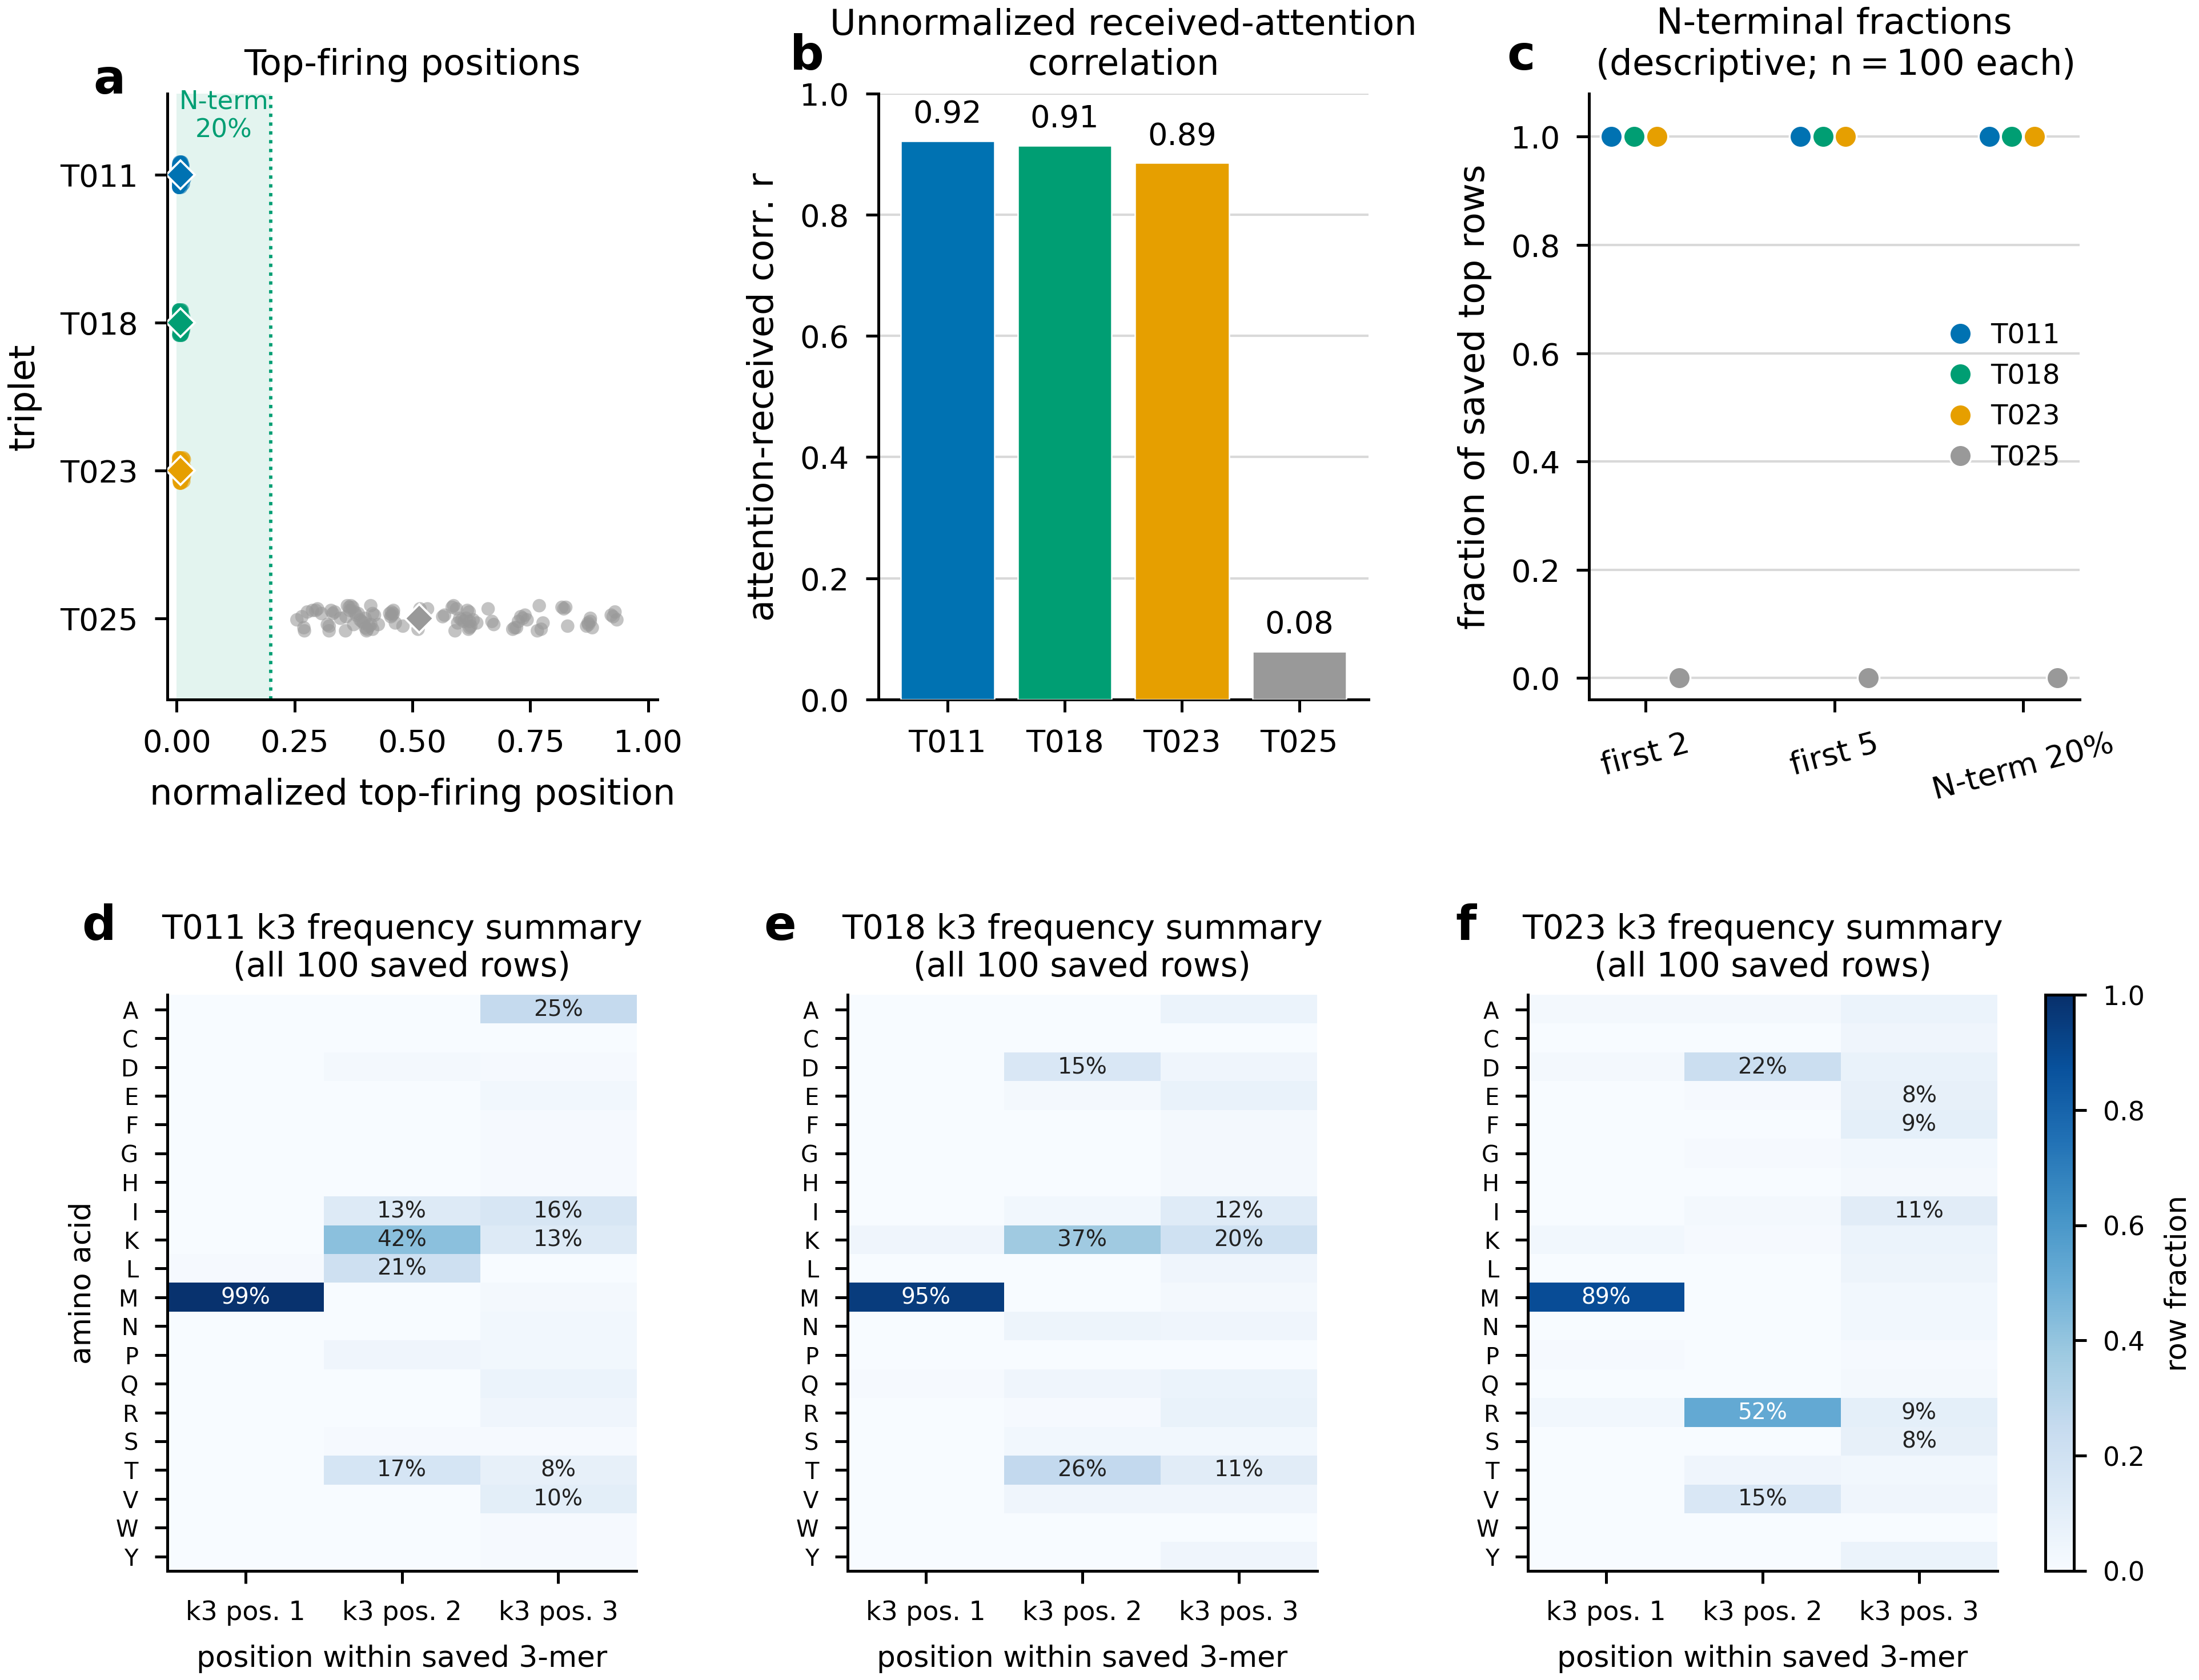
\includegraphics[width=\textwidth]{figures/figure_03_nterminal_readouts.pdf}
\caption{\textbf{Recurrent N-terminal sparse readouts.}
\textbf{a}, Normalized positions of the 100 saved top-firing rows per triplet; diamonds mark medians. \textbf{b}, Correlation with unnormalized same-layer received attention. Because early key positions can receive attention from more causal queries, this statistic is not a position-conditioned sink test. \textbf{c}, Descriptive fractions of saved top rows within the first two, first five and first 20\% of residues. \textbf{d--f}, Position-specific amino-acid frequencies across all 100 saved three-residue contexts for T011, T018 and T023. These panels summarize selected top events and are not estimates of population motif prevalence.}
\label{fig:sink}
\end{figure}

\subsection{Steering and ablation bound the causal evidence}

We next tested whether sparse readouts could act as control handles. Hook checks confirmed that the ZymCTRL MLP-output intervention path can move logits. These checks establish numerical reachability only; they do not show recovery of a known mechanism at realistic effect size, and the historical pipeline had no valid planted positive control. Candidate features from layers 3, 12 and 30 were then used to generate 100 steered and 100 unsteered sequences for each of eight enzyme classes. The selector requested five positive direct-effect candidates per class and layer but fell back to absolute-effect-ranked rows when fewer were available, introducing 19 negative-attribution interventions across six class/layer cells. Under a predeclared motif/composition score, no comparison met the positive statistical gate (Fig.~\ref{fig:negatives}a and Supplementary Table~7). The score is a heuristic placeholder rather than a validated EC classifier, and the sign defect prevents a clean positive-direction test. We therefore retain this run only as a no-positive-evidence pipeline pilot, not as evidence of biological failure of EC-class steering.

A separately evaluated 29 April lysozyme experiment used an older z-score-selected, off-manifold intervention and supplied external endpoints; it neither validates nor refutes the 3 May pilot above. Its generation-wide Pfam and CLEAN metrics did not establish an improvement over prompt conditioning: Pfam lysozyme-like hit rates were 0.860 for 200 steered and 0.820 for 200 unsteered sequences (one-sided Fisher $P=0.170$), and CLEAN exact EC 3.2.1.17 rates were 0.775 in both groups. Structural comparisons were available only for the post-selected ten steered leads and 20 unsteered sequences; mean local-ESMFold pLDDT was 67.7 versus 73.2 and mean Foldseek template-modelling score was 0.883 versus 0.938 (Fig.~\ref{fig:struct}d and Supplementary Table~8). Figure~\ref{fig:struct}a--c additionally shows older 17 April public-API structures and is a mixed-run historical illustration pending replacement. Structure display and lead selection were not blinded. Pfam, CLEAN, pLDDT and Foldseek are correlated computational filters rather than functional assays; experimental calibration work likewise shows that no single computational metric is universally sufficient to predict enzyme activity \cite{johnson2025computational}. The relevant positive-evidence gates were not met, but the mixed runs, unequal selected structural samples and computational endpoints do not establish a general lysozyme-steering negative or an eight-class biological verdict.

We also intervened on the N-terminal readouts and associated heads (Fig.~\ref{fig:negatives}b and Supplementary Table~9). TopK-aware MLP-output patching removed the CLT-explained component associated with T011, T018 or T023 and produced no consistent expected-direction effect across models. Single-head ablations targeted heads with high first-two-residue attention; top-8 and top-32 head-set ablations broadened the intervention. None met the joint likelihood, feature-drop and nominal matched-control gate. The available random controls were primarily layer matched, not uniformly matched on activation magnitude, decoder norm or received-attention mass. In the top-32 ZymCTRL run, random same-layer head sets changed likelihood more than the targeted set. An attention-output sparse pilot likewise failed its causal-damage gate. Thus, the specified causal claims remain unsupported under these interventions; the gate failures do not exclude every distributed or alternative-site mechanism, and feature/head discovery was not fully separated from evaluation.

The intervention matrix therefore defines an evidence boundary: recurrence and interpretable top events did not supply validated control handles under the tested paths.

\begin{figure}[t]
\centering
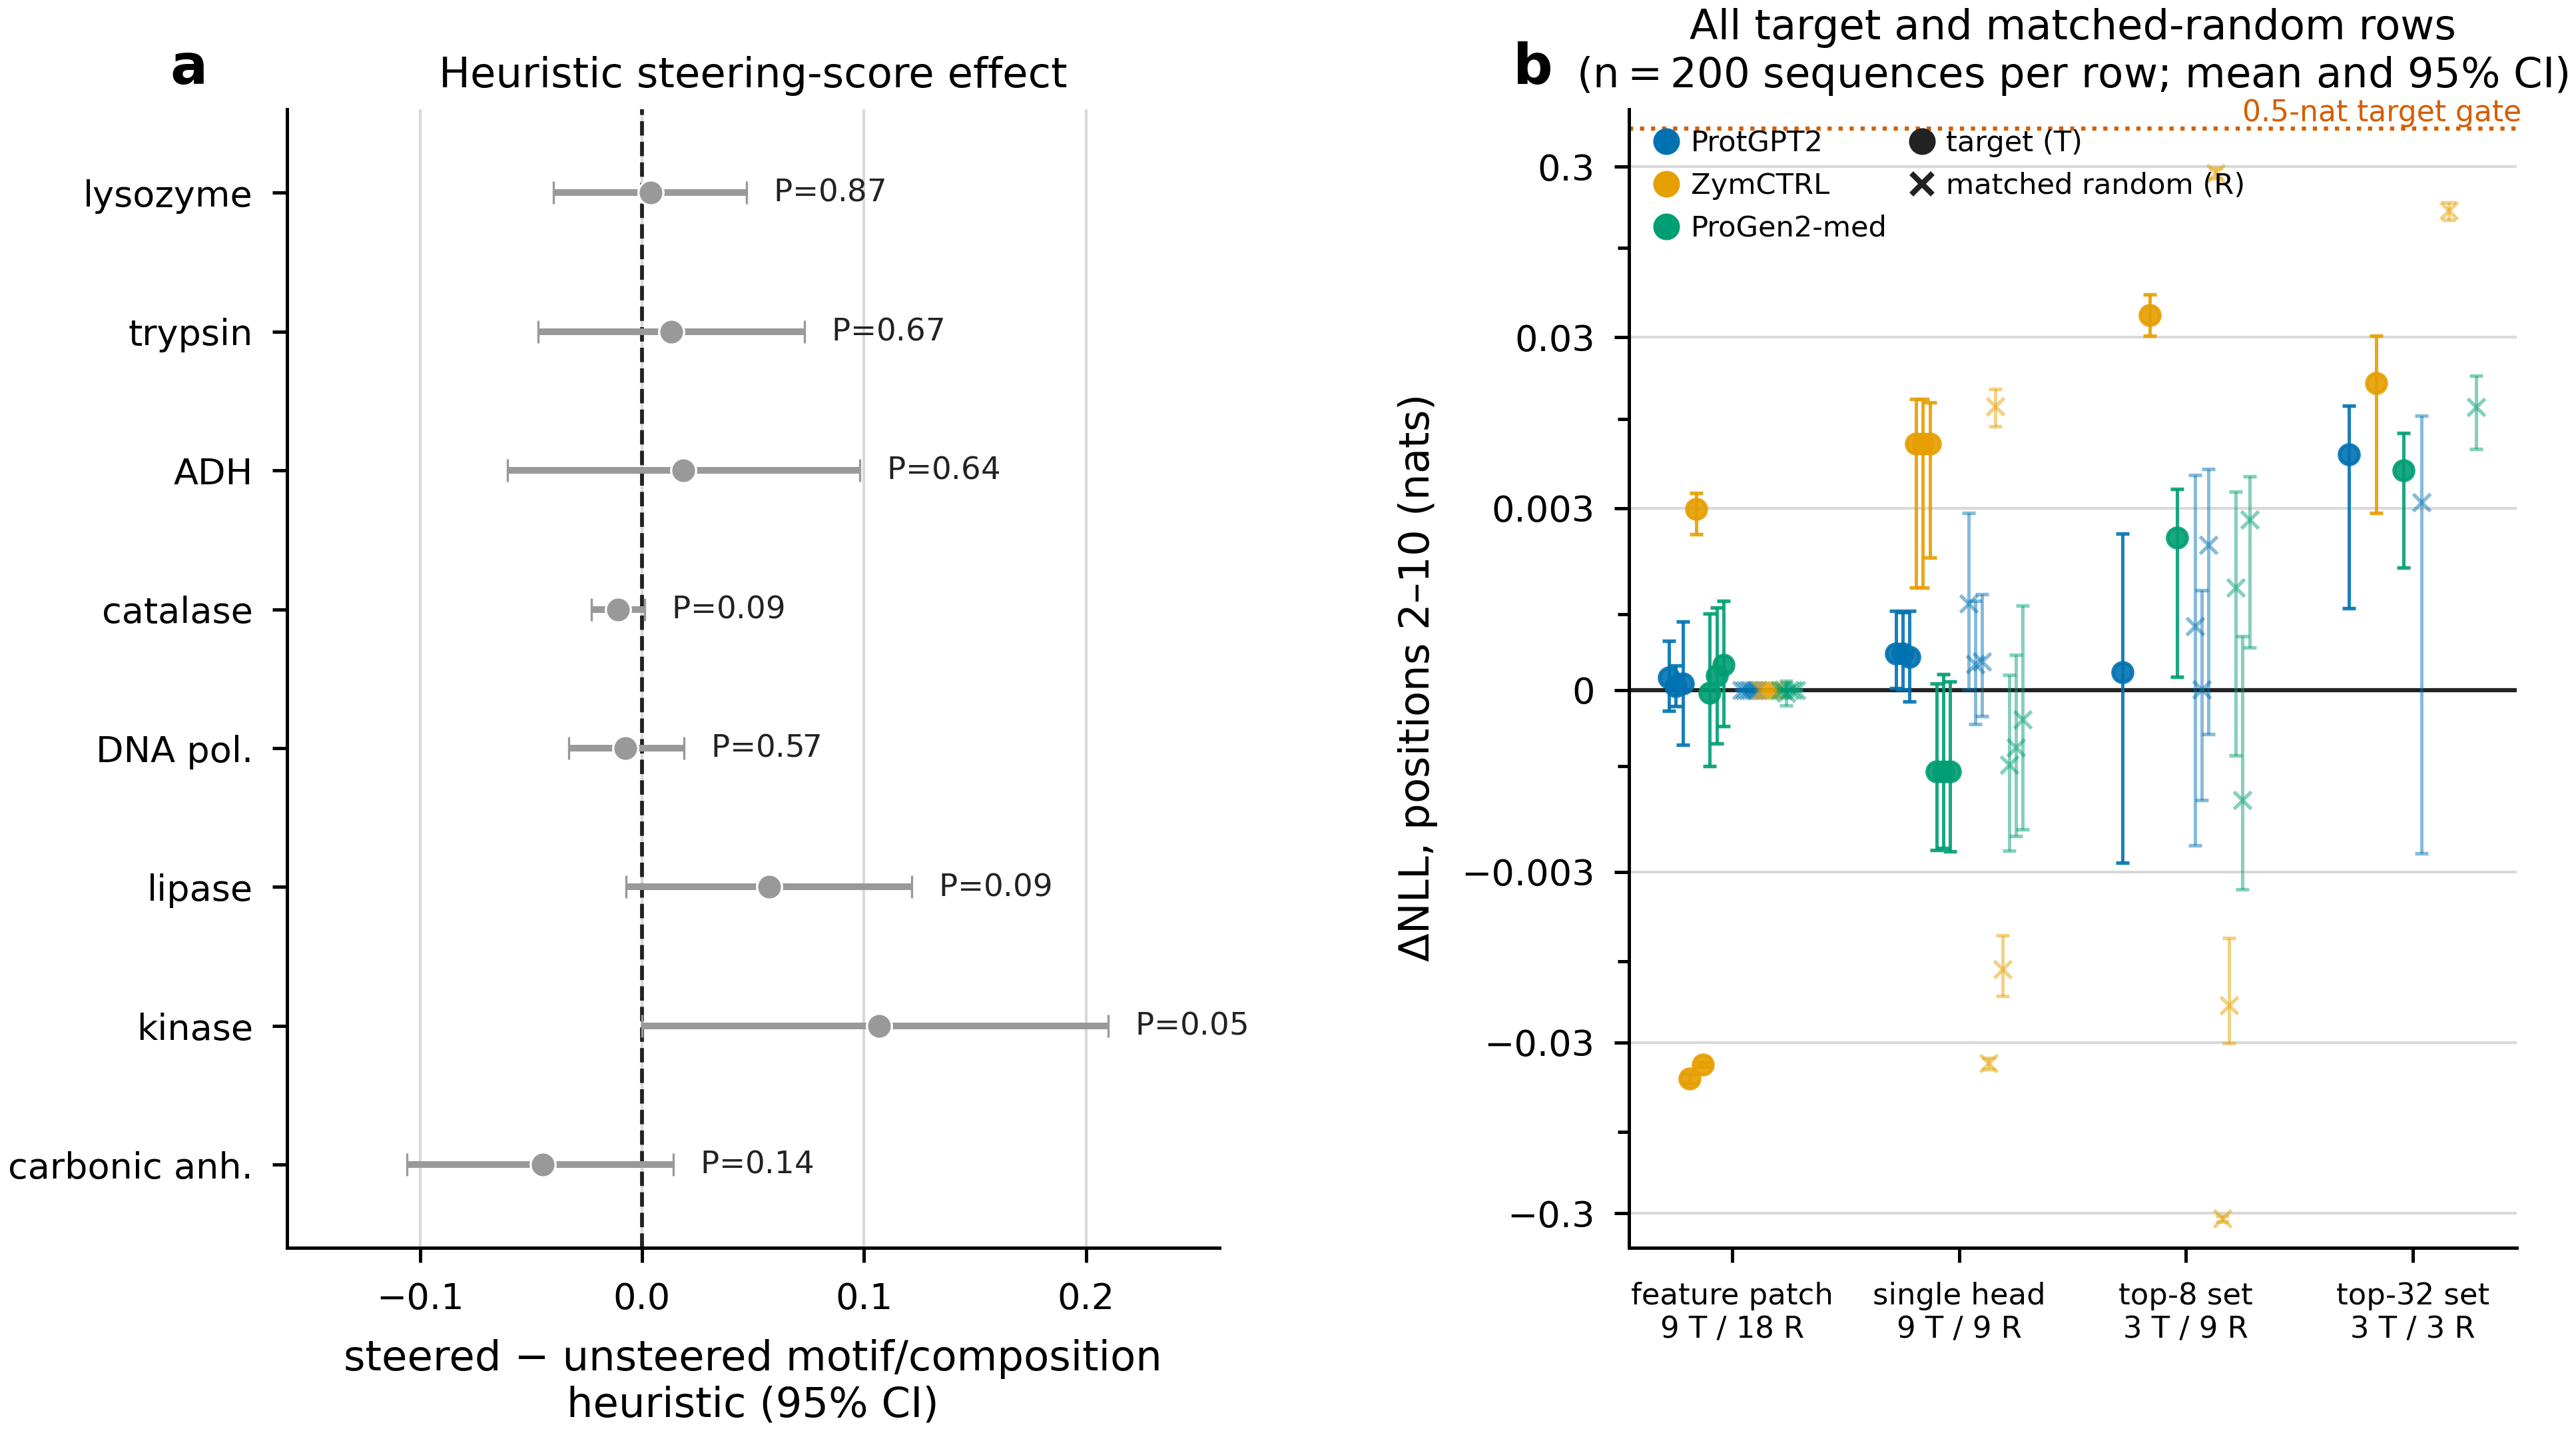
\includegraphics[width=\textwidth]{figures/figure_04_negative_interventions.pdf}
\caption{\textbf{The tested intervention paths do not validate causal control.}
\textbf{a}, Difference between steered and unsteered values of the predeclared motif/composition heuristic for eight ZymCTRL prompt classes, with 95\% bootstrap intervals and permutation $P$ values. This is not a validated EC-class score, and 19 of 120 selected interventions had negative attribution because of the fallback selector; the panel is a no-positive-evidence pipeline pilot, not a clean positive-direction negative. \textbf{b}, All 24 target and 39 available random-control $\Delta$NLL summaries at positions 2--10 for CLT-component patches, single-head ablations and top-8 or top-32 head-set ablations. Controls were primarily layer matched and were not uniformly matched on activation magnitude, decoder norm or received-attention mass. Each row contains 200 sequences; points and bars denote the mean and 95\% bootstrap interval on a symmetric-log scale. The panel reports the full saved set rather than selected maxima.}
\label{fig:negatives}
\end{figure}

\begin{figure}[t]
\centering
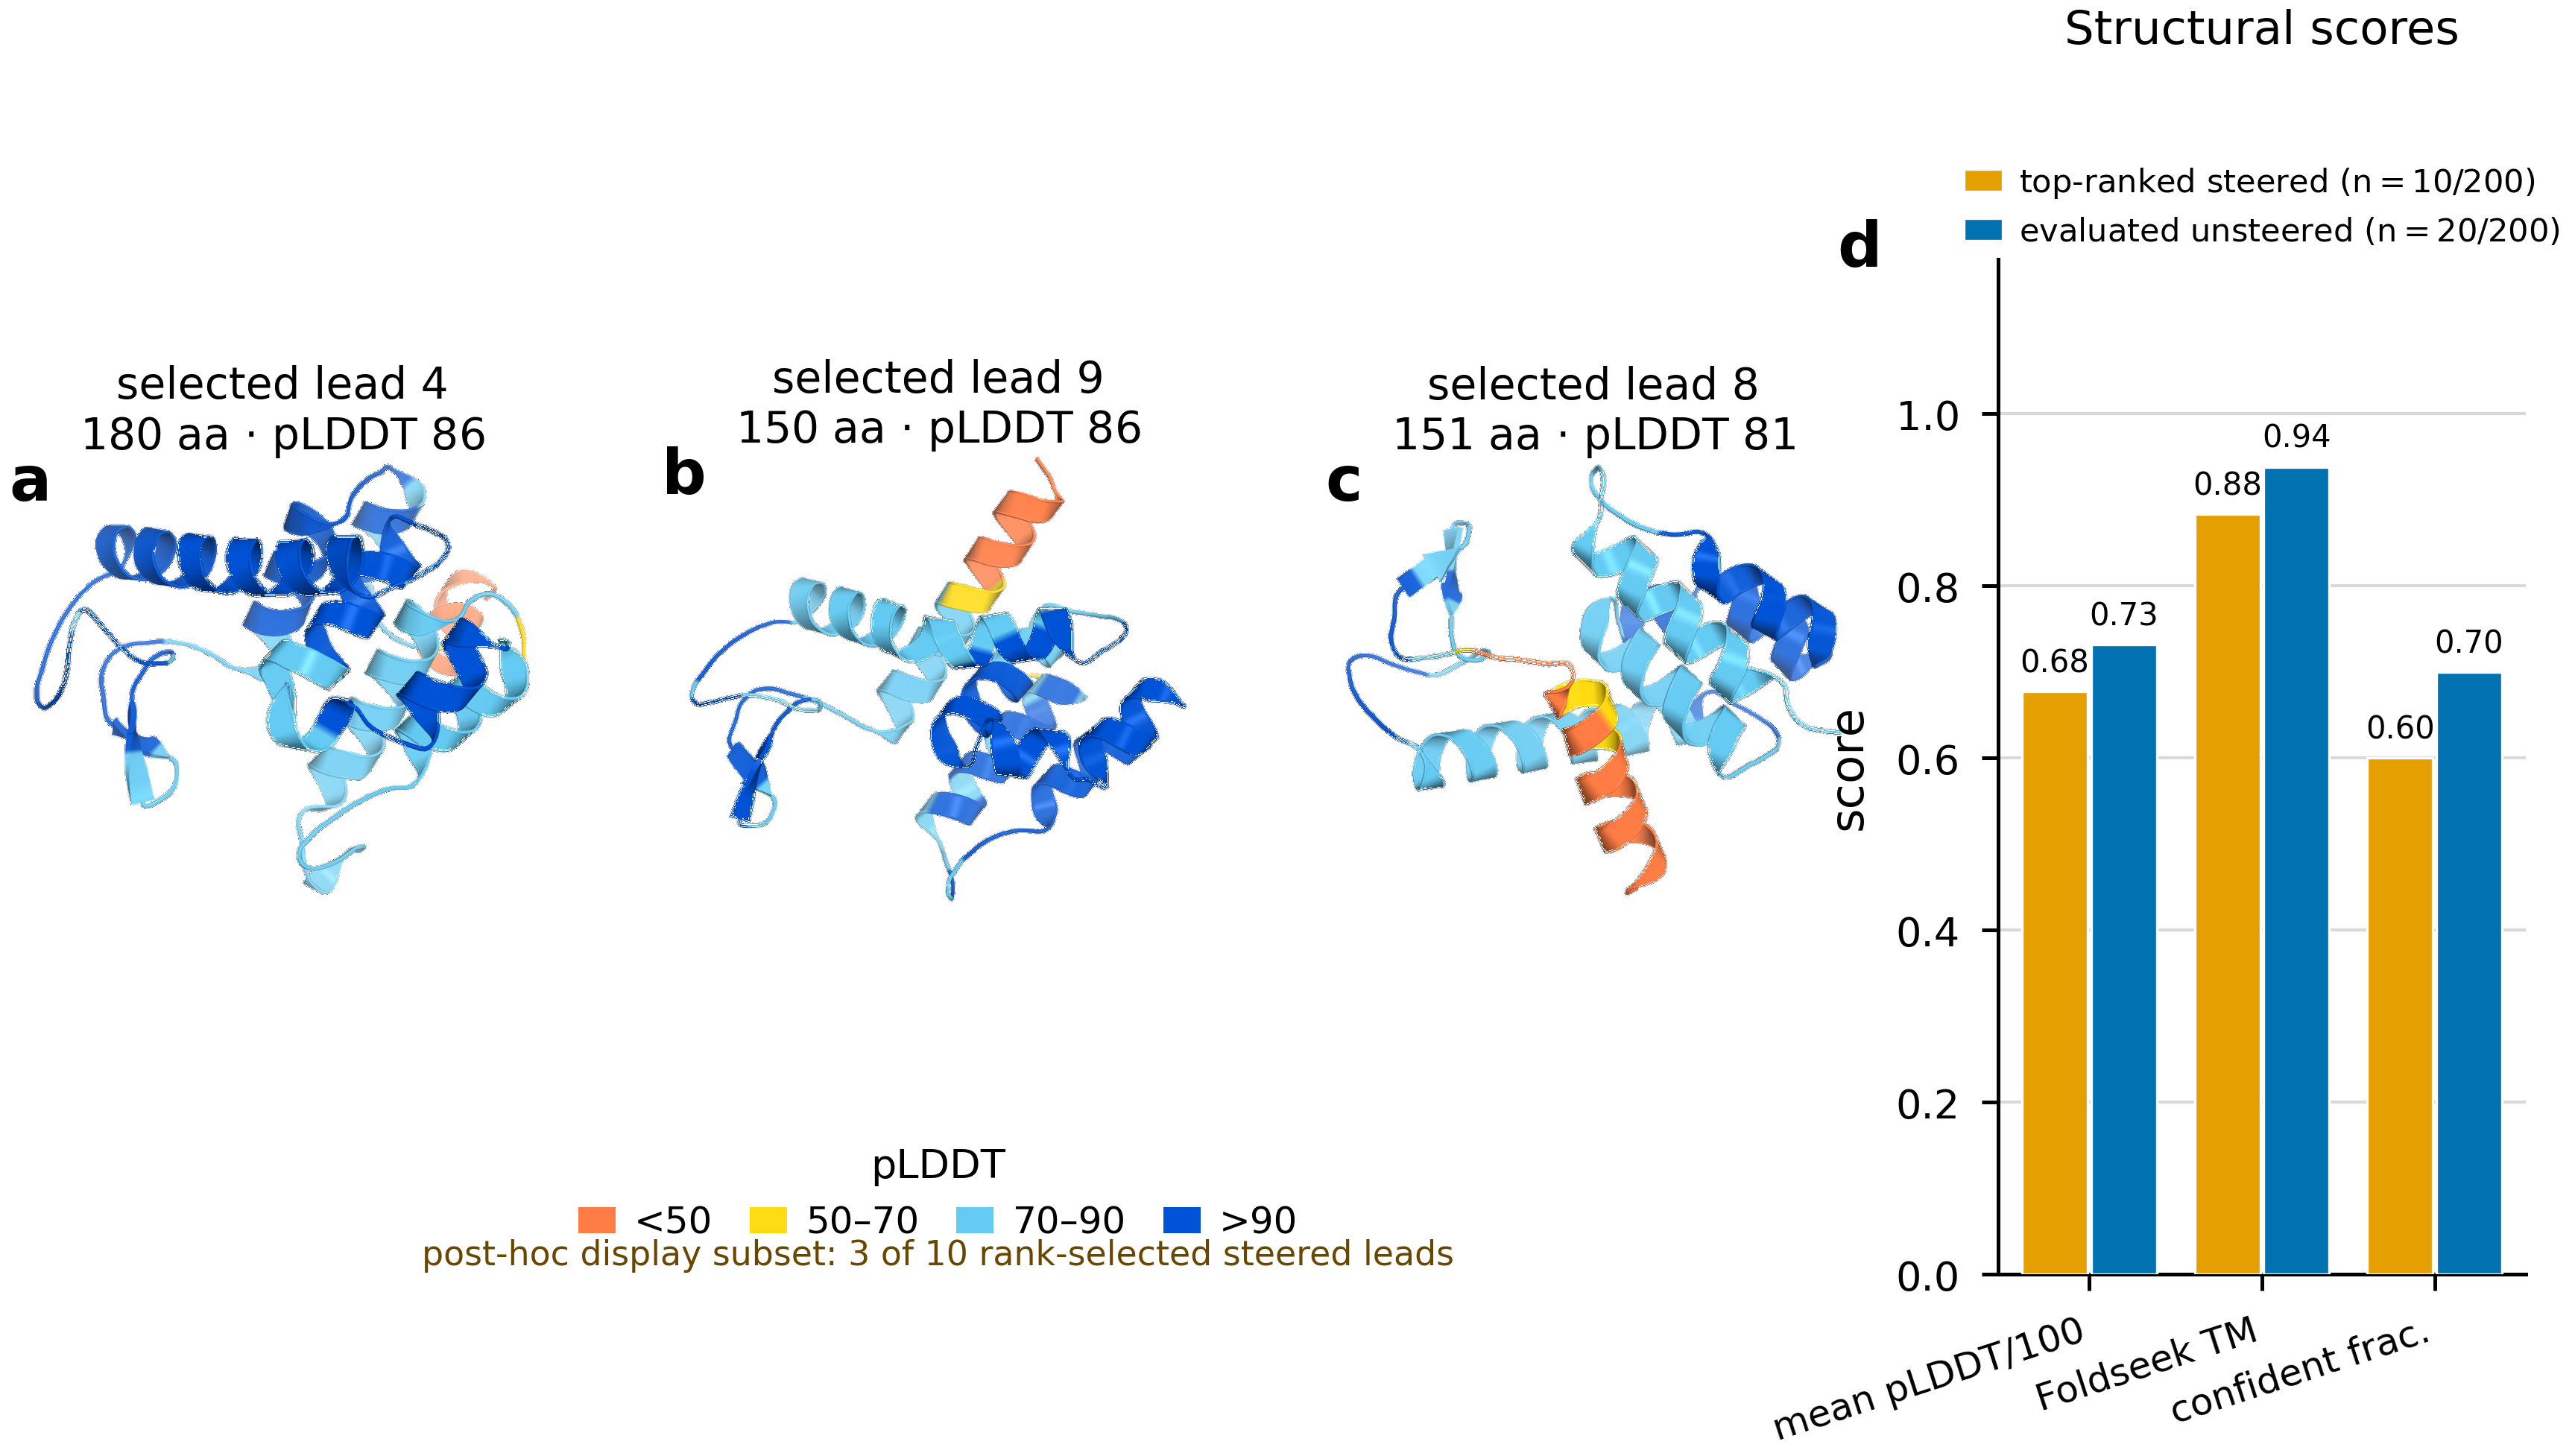
\includegraphics[width=\textwidth]{figures/figure_05_sequence_structure_checks.pdf}
\caption{\textbf{Historical lysozyme structures and provenance-bounded structural comparison.}
\textbf{a--c}, Three post-hoc high-pLDDT public-API display structures from a 17 April historical generation, shown as PyMOL cartoons and coloured by per-residue pLDDT. \textbf{d}, Local-ESMFold and Foldseek aggregates from a different 29 April z-score-selected/off-manifold generation: ten rank-selected steered leads and the first 20 unsteered prompt-conditioned sequences. Structure display and lead selection were not blinded. The panel therefore mixes historical runs and is retained only to disclose the existing evidence while a single-run symmetric replacement is prepared. No displayed structural endpoint favours the steered set; the unequal, selected samples preclude a general foldability claim and cannot evaluate the 3 May direct-effect pilot.}
\label{fig:struct}
\end{figure}

\subsection{A planted synthetic control calibrates the revised intervention pipeline}

To separate pipeline insensitivity from failure of a pretrained-model hypothesis, we prospectively froze and executed once a synthetic benchmark with three model seeds (11, 29 and 47), disjoint train, discovery and assessment splits of 48 sequences each, and no visible property-label token. A future W/Y endpoint was fixed to equality of canonical amino acids at zero-based positions 8 and 32. Each small autoregressive model exposed this relation through a seed-rotated, fixed sparse carrier/adapter path; this comparator was prescribed rather than learned as a biological circuit. A repository ReLU--TopK CLT was trained on the train split, candidate selection and control construction used the discovery split, and the assessment split was opened only afterwards (Supplementary Table~11).

The immutable production outcome passed the frozen synthetic gate. Each seed had sensitivity 1.0, specificity 1.0, false-discovery rate 0, endpoint accuracy 1.0 and a localized path. Effect-recovery ratios were numerically approximately 1.0 at doses 0.5, 1.0 and 2.0; all matched nuisance-direction and wrong-site effects met paired equivalence tests within the frozen $\pm0.50$ W/Y log-odds band. Assessment-set confound-adjusted activation Spearman correlations were 0.935, 0.998 and 0.946 across the three seed pairs. This result calibrates the revised synthetic CLT/intervention pipeline at the planted effect size only. It does not validate the historical controls, imply causality in ProtGPT2, ZymCTRL or ProGen2-medium, or close the real held-out pretrained-model target/control gate.

\subsection{Sparse codes retain selected linear signals under an amended audit}

We next asked whether the sparse codes retained information linearly decodable from the tensors on which the CLTs were trained. These tensors are architecture specific: the layer-normalized post-attention MLP input for ProtGPT2 and ZymCTRL, and the layer-normalized block input shared by attention and MLP for ProGen2-medium. They are not raw residual streams and are not homologous hook points across all three architectures. On 820 Swiss-Prot proteins (44{,}626 labelled residues; 48 ZymCTRL-conditioned sequences), we compared an L2-regularized probe on each selected CLT input (``ceiling'', $C$) with the same probe on its sparse code (``floor'', $F$), summarizing chance-corrected recovery as the clipped ratio $\rho=\operatorname{clip}(F/C,0,1)$ when $C>0$ (Fig.~\ref{fig:recoverability} and Supplementary Table~10). The analysis followed a preregistered protocol but incorporated logged post-result amendments, including fold-internal dimensionality reduction and exclusion of an unstable secondary-structure-fraction regression from decision gates.

CLT-input probes reached protein-family skill of 0.90--0.95, residue secondary-structure skill of 0.15--0.26 and ZymCTRL decoder-native EC skill of 0.65. Family-disjoint EC top-class ceilings were lower (0.12--0.27) than stratified ceilings (0.36--0.59), demonstrating substantial family dependence in this readout (Fig.~\ref{fig:recoverability}b). The sparse codes retained much of the selected signal for protein family ($\rho=0.85$--0.96), residue secondary structure ($\rho=0.81$--0.98) and ZymCTRL decoder-native EC ($\rho=0.81$). Recovery was lower for family-disjoint EC in ZymCTRL ($\rho=0.18$) and ProGen2-medium ($\rho=0.56$), so the audit does not support a uniform near-faithfulness claim.

The preregistered decision rule did not select a model for a capacity retrain. We nevertheless performed an explicitly exploratory override, training wider dictionaries at $d_\mathrm{CLT}=16{,}384$ for 300{,}000 steps. Recovery changes were mixed: ZymCTRL decoder-native EC rose from $\rho=0.81$ to 0.96 and ProGen2-medium family-disjoint EC from 0.56 to 0.84, whereas ProtGPT2 EC and Pfam recovery declined. None of the wider checkpoints met the preregistered FVU $<0.15$ criterion, and ProtGPT2 also missed the dead-fraction criterion. The runs therefore do not falsify dictionary capacity or optimization as contributors. Taken together, these analyses show that sparse codes can retain selected collective linear signals from their own inputs; they do not distinguish limitations of the model representations from dictionary optimization, feature geometry or intervention-space mismatch.

\begin{figure}[t]
\centering
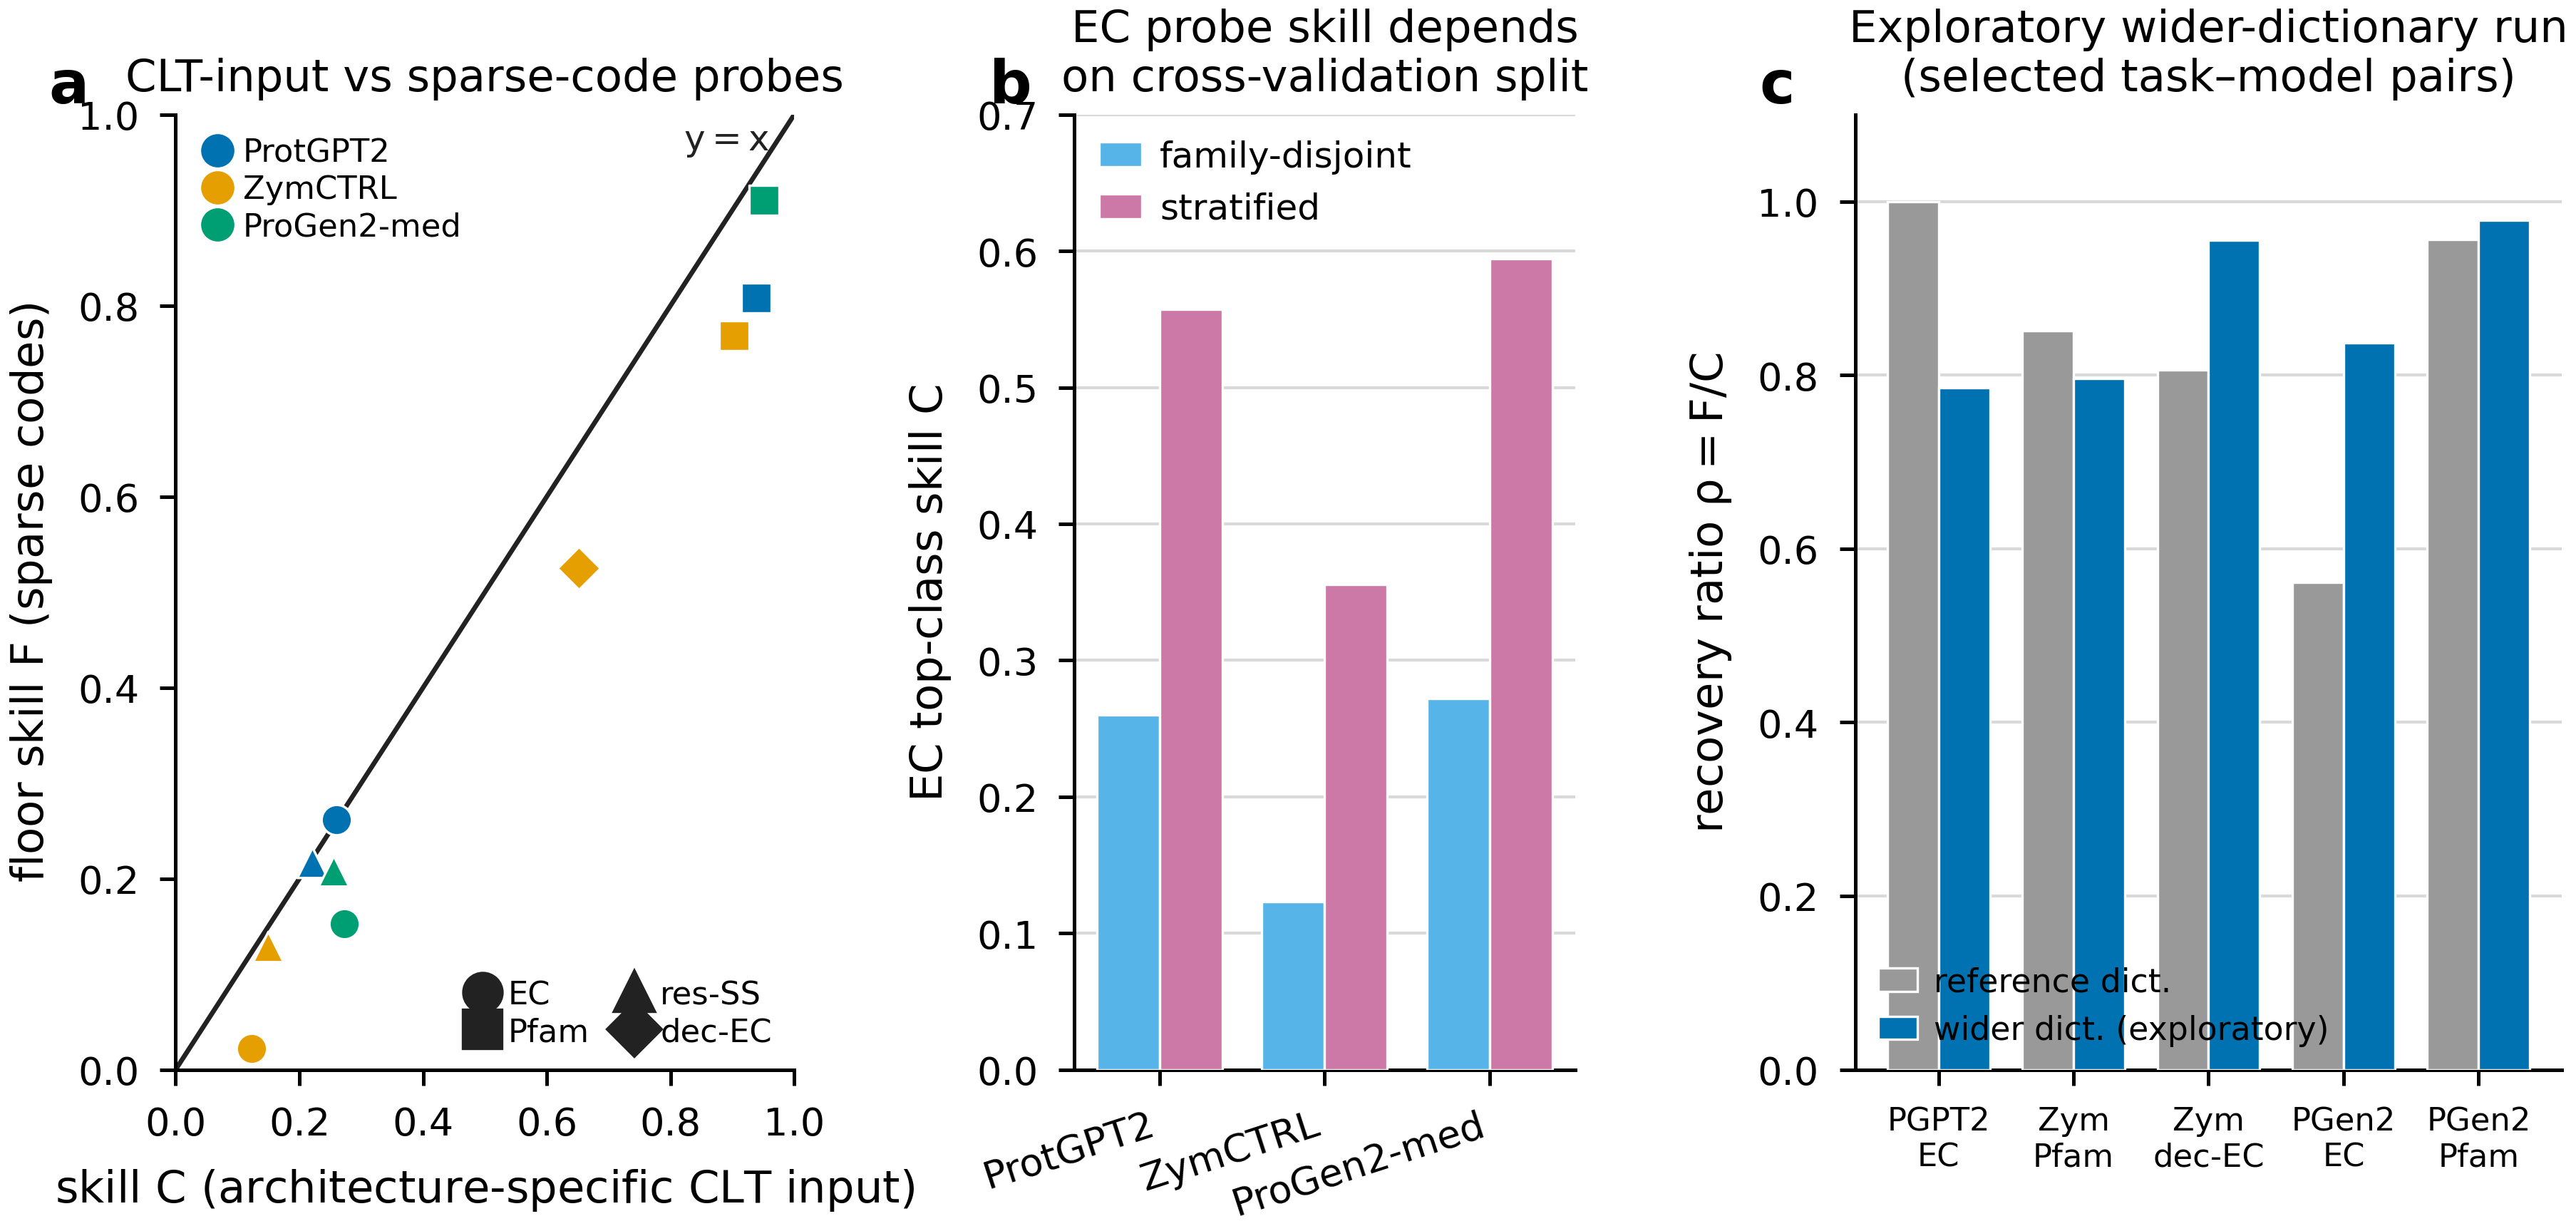
\includegraphics[width=\textwidth]{figures/figure_06_recoverability_audit.pdf}
\caption{\textbf{Selected linear-probe recovery from architecture-specific CLT inputs.}
\textbf{a}, Sparse-code floor skill $F$ versus CLT-input ceiling skill $C$ after the logged analysis amendments. The inputs are layer-normalized tensors at architecture-specific hook points, not raw residual streams. \textbf{b}, EC top-class ceiling under family-disjoint and stratified cross-validation, showing family dependence. \textbf{c}, Descriptive recovery ratios for reference and exploratory wider dictionaries. The wider checkpoints produced mixed changes and did not meet the preregistered reconstruction-quality criterion; the comparison therefore does not isolate capacity.}
\label{fig:recoverability}
\end{figure}

\section{Discussion}\label{sec:discussion}

Our results document a limited, procedure-specific descriptive observation: under one fixed cohort, layer mapping, variance filter and greedy matching rule, three protein generators contained 38 sparse-readout triplets above $|r|\geq0.90$, whereas 30 pair/layer-specific sequence reassignments produced at most one. Those reassignments were not coherent model-wise nulls. A separate 500-sequence UniRef50 cohort produced only eight triplets at 0.90 and no exact canonical feature identities, demonstrating cohort sensitivity rather than independent replication. The mature-versus-early comparison further shows that the statistic can be sensitive to training stage, but one checkpoint pair cannot validate it as a general quality metric. Testing additional trajectories, random seeds, coherent nulls and held-out protein cohorts is necessary before recurrent-triplet count can be used prospectively.

Recurrence did not resolve semantic status. Most triplets were associated with local sequence, position or CLT-input norm, and these associations overlapped. The original Swiss-Prot mutual-information gate was mathematically unattainable. Under its exploratory replacement, 0 of 380 associations met the Benjamini--Hochberg-adjusted $q<0.05$ gate for a within-protein amino-acid- and position-matched null, but only the previously selected top events were available and dominant Pfam was confounded with protein identity. The dimension-unmatched probe comparison likewise shows only that the selected 38-dimensional basis did not match the chosen ESM-2 representation. Neither analysis establishes an absence of biological information.

The N-terminal subset illustrates why descriptive and mechanistic evidence should remain separate. T011, T018 and T023 consistently marked initiator-methionine contexts and had high unnormalized received attention, yet early keys have more opportunities to receive causal attention. Feature patches, head ablations, larger head-set ablations and an attention-output sparse pilot all failed their specified joint gates. These gate failures bound the tested intervention family; they neither demonstrate a causal attention sink nor exclude mechanisms at other sites or scales. Numerical hook reachability was not a known-mechanism positive control, so the historical pipeline's sensitivity and effect-recovery calibration remain unknown. The prospectively frozen synthetic control shows that a revised pipeline can recover its fixed comparator at the planted effect size, but cannot retroactively calibrate those historical interventions or support a pretrained-model causal claim. The eight-class steering pilot used a motif/composition heuristic and contained a feature-sign selection defect. The external Pfam, CLEAN and structure endpoints came from a separate older lysozyme intervention and did not meet positive-evidence gates; they cannot validate or refute the later pilot.

The amended recoverability audit narrows a different uncertainty. Sparse codes often retained selected linear signals available in their own CLT-input tensors, but recovery was not uniformly high and the hook points were not homologous across all architectures. The exploratory wider dictionaries produced gains for some readouts and losses for others; none satisfied the preregistered reconstruction-quality requirement. These analyses therefore do not attribute the intervention gate failures to model substrate, dictionary capacity, optimization, feature geometry or hook-site mismatch. They show only that width alone did not yield a consistent improvement in the evaluated linear readouts.

Several limitations constrain generalization. We examined three decoder models, three anchor depths, a 200-sequence matching cohort and the 4,096 highest-variance candidates, with discovery and assessment performed on overlapping saved outputs. ProtGPT2 and ZymCTRL share a GPT-2-family architecture, ProGen2-medium is the sole major architectural contrast, and the CLT hook sites are not homologous. Architecture, training corpus and tokenizer therefore remain entangled rather than factorially separated. The historical balanced-cohort file has been recovered from archived compute storage but is not yet in a public deposit; CLT training and quick evaluation included padded positions, several residue-level nulls did not preserve protein clustering, head discovery was not fully separated from evaluation, the dictionaries were not seed-replicated, and no wet-laboratory assay was performed. A useful benchmark for decoder interpretability should therefore require immutable cohort manifests, protein-blocked nulls, mask-aware dictionary evaluation, external biological endpoints and held-out intervention controls. Cross-model recurrence can be one diagnostic in that benchmark, but semantic and causal claims require independent gates.

\section{Methods}\label{sec:methods}

\subsection{Models and sparse dictionaries}

We analysed frozen local copies of the published ProtGPT2, ZymCTRL and ProGen2-medium checkpoints \cite{ferruz2022protgpt2,munsamy2022zymctrl,nijkamp2023progen2}. ProtGPT2 and ZymCTRL are 36-layer GPT-2-family models with hidden size 1,280 and 20 attention heads; ProGen2-medium (upstream identifier \texttt{hugohrban/progen2-medium}) has 27 layers, hidden size 1,536 and 16 heads and supplies the panel's sole major architectural contrast. ProtGPT2 uses a multi-residue BPE vocabulary, whereas ZymCTRL and ProGen2-medium use residue-level vocabularies; the models also differ in training corpus. Architecture, corpus and tokenizer effects are consequently entangled. A deployment-tree audit established three different provenance states. The complete deployed ProtGPT2 model/tokenizer tree is verified against Hugging Face commit \hashvalue{f71aa6cf063ad784ebd53881d11332fd098eaa58}. ZymCTRL is best supported at upstream revision \texttt{3c532ef...}, and its deployed weight file is verified, but strict proof that the complete deployed model/tokenizer tree matches that revision remains incomplete. The deployed ProGen2-medium tree is a hybrid with no single upstream commit; exact reproduction therefore requires a deposited local file manifest and snapshot rather than assignment of one upstream revision. These provenance recoveries do not complete the public archive or close P0-1.

Each CLT encoded an input tensor $x_l$ at source layer $l$ as $z_l=\operatorname{TopK}_k[\operatorname{ReLU}(W_lx_l+b_l)]$. A windowed decoder reconstructed the MLP output at target layer $t$ from features in the preceding eight-layer window, and training minimized mean squared reconstruction error averaged over target layers. ProtGPT2 and ZymCTRL reference dictionaries used all 36 layers, $d_\mathrm{CLT}=8192$, $k=128$ and 200,000 steps. The ProGen2-medium atlas checkpoint used all 27 layers, $d_\mathrm{CLT}=4096$, $k=64$ and 100,000 steps. One reference dictionary per model supplied the historical atlas; no dictionary-seed replication was performed. ProtGPT2 was trained from UniRef50 sequences and ZymCTRL from EC-labelled sequences, with maximum tokenized length 256; configuration files record the remaining optimizer and sampling settings.

The hooked tensor $x_l$ was the layer-normalized post-attention MLP input in ProtGPT2 and ZymCTRL, but the layer-normalized block input shared by attention and MLP in ProGen2-medium. Accordingly, we call it the architecture-specific CLT input rather than a raw residual stream. Batched CLT training and quick evaluation did not pass the tokenizer attention mask into the model or exclude padded positions from loss and feature statistics. Reconstruction of the saved 100-sequence quick evaluations found 298 of 8,342 padded positions (3.57\%) for ProtGPT2 and 673 of 24,466 (2.75\%) for ZymCTRL. Single-sequence atlas extraction contained no right padding. We report fraction of variance unexplained (FVU) and dead-feature fraction as unmasked diagnostics.

\subsection{Cross-model triplet atlas}

The atlas used a fixed balanced set of 200 protein sequences truncated to 256 residues. For each sequence and selected layer, token-level sparse activations were mean-pooled to obtain one activation per feature. Anchor layers 5, 12 and 30 in the 36-layer models were mapped by relative depth to layers 4, 9 and 22 in ProGen2-medium. Within each model and layer, the 4,096 features with highest across-sequence variance formed the candidate pool. Pairwise absolute Pearson correlations were greedily matched one to one, retaining the top 300 pairs. An exact triplet required all three pairwise edges to exceed the stated threshold. This selection and matching procedure was not optimized or evaluated on an independent cohort. A development run on 500 UniRef50 sequences yielded eight and three exact triplets at thresholds 0.90 and 0.95, respectively, with no exact feature-identity overlap with the canonical set.

For the null, the sequence order of one member of each model pair was independently permuted at each layer before repeating feature matching and exact-triplet enumeration. Thus, the three edges closing a null triangle could arise from different reassignments; this is a pair/layer-specific null rather than one coherent model-wise permutation. We used 30 replicates with seed 20260513 and thresholds 0.90, 0.95 and 0.98. During the initial audit, the original balanced-cohort JSON was absent from the working mirror, so we reconstructed 200 records by preserving the retained within-source orders and interleaving the 100 real lysozyme and 100 random UniRef50 records according to the documented alternating rule. We subsequently recovered from archived compute storage the exact historical file named by the saved atlas provenance (file SHA-256 \hashvalue{5bc7697a83cc7461558f8b4597a3c9b4d6a151b7ec70ca22efc7282ecde4f0a6}). Its ordered records exactly equal the reconstruction before added provenance fields. The enriched ordered-record SHA-256 is \hashvalue{07213d4a9cefbdb055206e08d3137722c446acf43b5b3342db571b977032c724}, with local status \texttt{historical\_exact\_file\_verified}. We also located and hash-verified the three exact reference CLT files named by the saved atlas output; their identities and retained configurations are recorded in the accompanying recovery manifest. Exact regeneration still requires strict whole-tree provenance for ZymCTRL, a deposited local file manifest and snapshot for the hybrid ProGen2-medium deployment, complete execution metadata and deposition of the recovered inputs.

\subsection{Swiss-Prot annotation re-audit and basis probes}

The original annotation analysis selected 500 Swiss-Prot proteins of length 100--400 residues by round-robin sampling over dominant Pfam labels \cite{uniprot2025,mistry2021pfam}. For each triplet it binarized the 100 highest-scoring positions among 122,671 valid positions and calculated plug-in mutual information against ten label families. Because the binary event prevalence was $100/122{,}671$, its entropy and hence its maximum possible mutual information was 0.00661255 nats; the original 0.1-nat gate was invalid and was removed.

We reanalysed the 3,800 retained top events using normalized mutual information $I(B;L)/H(B)$. Two thousand global null replicates sampled 100 positions without replacement. Two thousand matched replicates preserved protein and amino-acid identity and matched exact N- or C-terminal edge classes or normalized-position ventiles. Upper-tail permutation $P$ values used the plus-one correction and were adjusted by the Benjamini--Hochberg procedure across 38 triplets and ten label families (380 tests). The deterministic reanalysis used seed 20260716. It is exploratory because it was designed after auditing the gate and continuous activations were unavailable.

The downstream basis analysis compared the 38-dimensional triplet representation with 2,560-dimensional mean-pooled ESM-2 embeddings on Pfam-family classification, EC top-class classification and secondary-structure-fraction regression. The saved implementation used record-level stratified folds for classification and record-level folds for regression, with different random seeds and folds across the two representation arms; stronger family-aware wording was not implemented. Because folds, representation dimension and model class were not matched, we treat the comparison as descriptive.

\subsection{Triplet characterization}

Characterization combined the 500-protein Swiss-Prot cohort with 200 calibration sequences. Per-model activation values were standardized over all retained cohort positions and then averaged across the three matched features at aligned residue positions. For each triplet, the 100 highest consensus values defined saved top events. Five tests evaluated centred 3- or 5-mer enrichment, normalized position, ProtGPT2 BPE-boundary enrichment, Pearson correlation with same-layer received attention and Pearson correlation with CLT-input L2 norm. Received attention was averaged across heads and queries for each key position and was not divided by the number of eligible causal queries.

Each test used 2,000 implemented permutations, and the resulting values were adjusted by Benjamini--Hochberg across 38 triplets and five test families. These permutations generally treated residue positions as exchangeable rather than preserving proteins. In addition, the smaller $P$ value from the 3-mer and 5-mer tests was selected without a second selection correction. The tests are therefore exploratory. For the N-terminal summary, top-event sequence identifiers were checked to establish that each of T011, T018 and T023 represented 100 different proteins rather than repeated positions from a few proteins.

The checkpoint comparison repeated the atlas procedure for the mature reference pair and a 10,000-step ProtGPT2/ZymCTRL pair while leaving ProGen2-medium fixed. No additional training seeds or intermediate checkpoints were tested.

\subsection{Historical TopK-aware steering pilot}

ZymCTRL enzyme-class steering requested five positive direct-effect features from each of layers 3, 12 and 30 and used a multiplier of 2.5. Candidate rows had first been ranked by absolute direct effect. When fewer than five positive rows were present among the ten saved candidates, the selector fell back to the first five absolute-ranked rows; 19 of 120 selected interventions were consequently negative-attribution features across six class/layer cells. The hook recomputed the TopK code after changing the selected preactivations and replaced the CLT-explained MLP component. For each of eight prompts, 100 steered and 100 unsteered sequences were generated. The primary score was a predeclared collection of class-specific motif and amino-acid-composition rules implemented as \texttt{ec\_purity\_score}; it is a heuristic pipeline score, not a trained or externally validated EC classifier. Mean differences used 10,000 bootstrap replicates for 95\% intervals and 10,000 label permutations for two-sided permutation $P$ values. Because of the selection defect, this historical run is not a clean positive-direction steering test.

\subsection{External sequence-quality metrics}

The 29 April lysozyme case study used prompt \texttt{3.2.1.17<sep><start>} and a z-score-selected/off-manifold intervention distinct from the 3 May direct-effect pilot. Generated sequences were evaluated with Pfam/HMMER domain hits \cite{mistry2021pfam,potter2018hmmer}, CLEAN EC prediction \cite{yu2023clean}, local ESMFold structural prediction \cite{lin2023esm} and Foldseek similarity \cite{vankempen2024foldseek} against the staged structure database. A real-versus-random calibration was completed retrospectively after the generated metric triad. Pfam and CLEAN covered 200 steered and 200 unsteered generations. Local ESMFold and Foldseek covered ten post-selected steered leads and 20 unsteered sequences, so the structural comparison is neither randomized nor generation-wide. The three structures in Fig.~\ref{fig:struct}a--c instead came from a still older 17 April public-API run. Neither the post-hoc display selection nor the 29 April steered-lead rank selection was blinded; the mixed-run display is historical provenance, not one efficacy experiment.

\subsection{Causal and intervention analyses}

The CLT feature patch used TopK-aware same-layer MLP-output patching for T011, T018 and T023. This subtracts the decoder contribution attributed to an encoded CLT component; it is not literal deletion of a neuron or of the full model state. Direct attention-head ablation zeroed selected head-output slices before the attention output projection. Head-set experiments applied the same operation to the top-8 or top-32 N-terminal candidates and sampled same-layer random head sets. These random controls were chiefly layer matched; they were not uniformly matched on activation magnitude, decoder norm, received-attention mass or other target properties. The attention-output pilot trained a sparse dictionary on the input to the ZymCTRL attention output projection and ablated its highest-ranked N-terminal readout. Feature-, head- and head-set per-sequence effects were summarized with 1,000 bootstrap resamples; the saved attention-output pilot retained plain means rather than bootstrap intervals. A positive gate required the expected direction, readout damage and specificity beyond the available control, but the limited matching weakens that specificity test. Selection and evaluation data were not fully independent.

\subsection{Prospective planted synthetic control}

The prospective calibration used only BOS, EOS and the 20 canonical amino acids as model-visible tokens. Equality of A/C residues at zero-based positions 8 and 32 determined a future W/Y endpoint; both anchor marginals and the target state were balanced independently within train, discovery and assessment splits. Motif identity, motif position, length, family and N-terminal state were also balanced, and equality relations at positions 10/34 and 12/36 supplied two active nuisance mechanisms. The frozen production specification used three model seeds (11, 29 and 47), 48 records per split, a two-layer causal autoregressive model and a 10-coordinate ReLU--TopK CLT with $k=3$. A seed-specific rotation concealed a fixed carrier/adapter path whose W/Y effect was prescribed. The comparator therefore provides known synthetic causal truth but is not an emergent biological mechanism.

Model and CLT fitting used only the training split. Discovery fitted a prespecified conditional activation model adjusting for motif, motif position, length, k-mer count, family, N-terminal state, both target-anchor states and both nuisance relations. Candidate coordinates required a positive conditional coefficient, one-sided Benjamini--Hochberg-adjusted $q<0.05$ and the frozen direct-effect threshold. Control construction then matched the two orthogonal nuisance directions at the target layer and site on firing frequency, mean activation, decoder norm, general direct-logit-effect norm, received attention and reconstruction contribution, with fixed component calipers and no fallback. Only after fitting, selection and matching were complete was the assessment split used for endpoint accuracy, CLT FVU, localization, three-dose recovery, wrong-layer and wrong-position effects, matched-control effects and cross-seed activation alignment.

The per-seed gate required sensitivity $\geq0.80$, specificity $\geq0.95$, false-discovery rate $\leq0.10$, endpoint accuracy $\geq0.80$, mean and layer-1 FVU $\leq0.50$, path localization and dose recovery in $[0.80,1.20]$. Every seed pair required confound-adjusted activation Spearman correlation $\geq0.80$. Wrong-layer, wrong-position and nuisance-direction effects at doses 0.5, 1.0 and 2.0 had to pass paired two-one-sided equivalence tests at $\alpha=0.05$ inside $[-0.50,0.50]$ W/Y log-odds. The specification was frozen before production execution and the exclusive execution claim prohibited retry or retuning. The immutable spec, freeze-manifest, execution-claim, summary and run-manifest SHA-256 values are, respectively, \hashvalue{6adb9377d732c0f126191767f1573a62850e08cea04e63e45090cee1c9829167}, \hashvalue{c8ece12dfecf1eefdafb2436ad39220d0c3c5f11e2f7a331fb712e956f0774e3}, \hashvalue{32e2e12156fb733414d3ee0ab556a6d131f979cd8240d03ce1161eee04ab6e93}, \hashvalue{d952a75dc2785d305bd245c6e79b0e7fc94122c475af3ecadd08d3411962dbea} and \hashvalue{930ad2d4fbcbee63568cd52a9c4209b2270727c6b9b8fd446a2d0044450ef039}.

\subsection{Representation-recoverability audit}

The recoverability protocol was frozen on 4 June 2026 and its subsequent validity amendments were logged. The cohort contained 820 Swiss-Prot proteins, 44,626 labelled residues and 48 ZymCTRL-conditioned generated sequences. For each selected layer we extracted the architecture-specific CLT input ($C$), the sparse code at the same layer ($F$) and, where available, the CLT reconstruction. Protein-level arrays were mean-pooled; secondary structure was evaluated per residue. Tasks were EC top-class, Pfam family, residue secondary structure and ZymCTRL decoder-native EC. The protein-level secondary-structure-fraction regression was retained as report-only after numerical instability was identified.

Classification used L2-regularized logistic regression and regression used ridge regression. Standardization and principal-component reduction to at most 256 dimensions were fitted within each training fold. EC top-class used fivefold family-disjoint cross-validation and was also reported under stratified cross-validation to quantify family leakage; Pfam-family classification and decoder-native EC used stratified folds. The best CLT-input layer was selected from the same cross-validated cohort, and the sparse-code score was then evaluated at that layer. Skill was macro-F1 minus an empirical shuffled/majority reference for classification and $R^2$ for regression. The reported recovery ratio was $\rho=\operatorname{clip}(F/C,0,1)$ when $C>0$; clipping prevents negative ratios or values above 1 from being interpreted as negative or super-recovery. Confidence intervals used 1,000 group-level bootstrap resamples of the out-of-fold predictions. The preregistered five-seed repetition and multiplicity analysis across layers were not completed, so the audit is descriptive rather than a confirmatory hypothesis test.

The preregistered decision rule returned no-go for a capacity retrain. An exploratory override nevertheless trained all three dictionaries at $d_\mathrm{CLT}=16{,}384$, $k=128$ for 300,000 steps and repeated the probes. This was approximately twofold wider for ProtGPT2 and ZymCTRL and fourfold for ProGen2-medium. Final recorded FVU/dead fractions were 0.278/0.334, 0.335/0.044 and 0.310/0.122, respectively. None met the preregistered FVU $<0.15$ requirement for a demonstrably better dictionary, and the quality values were not obtained in a matched held-out evaluation. We report recovery changes descriptively and do not use the mismatched input-derived/output-injected direction experiment for a controllability conclusion.

\subsection{Statistics}

Exact sample sizes, resampling counts and statistical units are given above and in the source-data tables. Atlas nulls used sequences as the permuted unit but drew independent reassignments for each pair/layer edge. The annotation re-audit used upper-tail permutation tests; steering used two-sided label permutations; the preregistered Pfam lysozyme comparison used a one-sided Fisher exact test. Unless stated otherwise, confidence intervals are percentile bootstrap intervals; the attention-output pilot is an exception because its saved summary contains means only. Triplet characterization and the annotation re-audit used Benjamini--Hochberg correction over their stated test families. Characterization tests that did not preserve protein identity are labelled exploratory. The prospective synthetic calibration froze its $\pm0.50$ log-odds equivalence region and paired two-one-sided tests before execution. No prospective power calculation or equivalence region was specified for the historical analyses; their sample sizes followed the frozen cohorts or the available staged outputs. The deterministic analyses were not blinded, and the historical Figure~\ref{fig:struct} structure display and steered-lead selection were explicitly post hoc and unblinded. No intervention was considered positive without the specified direction and available-control criterion; the historical random controls were not uniformly matched beyond layer.

\subsection{Use of generative AI tools}

During manuscript preparation, the authors used OpenAI Codex to assist with literature organization, LaTeX restructuring and language editing. The authors reviewed the scientific claims, calculations, citations and generated text and take responsibility for the submitted content.

\section*{Data availability}

The accompanying \texttt{source\_data} directory contains processed tables and JSON summaries for the empirical Figs~\ref{fig:atlas}--\ref{fig:recoverability} and Supplementary Tables 1--11, together with a file manifest and SHA-256 checksums. The Supplementary Table~11 package includes the exact frozen specification, freeze manifest, execution claim, result summary and run manifest for the prospective synthetic calibration, plus a deterministic per-seed numeric extraction; its summary and run-manifest SHA-256 values are \hashvalue{d952a75dc2785d305bd245c6e79b0e7fc94122c475af3ecadd08d3411962dbea} and \hashvalue{930ad2d4fbcbee63568cd52a9c4209b2270727c6b9b8fd446a2d0044450ef039}. Figure~\ref{fig:workflow} is a conceptual proposal and has no empirical source dataset. For Fig.~\ref{fig:struct}, the package contains aggregate metrics and run/source hashes but not the rendered structures, underlying generated sequences or a panel-complete single-run experiment. A machine-readable historical panel/table map separately records which upstream commands, revisions or checkpoints remain unavailable; those missing fields are not treated as reproduced provenance. Swiss-Prot, UniRef, Pfam and the pretrained model weights are available from their cited public sources subject to their source licences. The recovered historical 200-record cohort file has SHA-256 \hashvalue{5bc7697a83cc7461558f8b4597a3c9b4d6a151b7ec70ca22efc7282ecde4f0a6}; its enriched ordered records have SHA-256 \hashvalue{07213d4a9cefbdb055206e08d3137722c446acf43b5b3342db571b977032c724} and local status \texttt{historical\_exact\_file\_verified}. Because it is sequence-bearing, it is not included in the compact processed package and must be placed in the final licensed deposit. The three historical reference CLT files have likewise been located and hash-verified on archived compute storage: ProtGPT2 \hashvalue{5eca3b19284dbd9b302078e3a7e34ce7a2fc78d97b1566eae927d4d1c30f1f00}, ZymCTRL \hashvalue{5da70c530b83a034d1fe683a72a8cc5bd7b49463d2598036cd6b5db94ca5761d} and ProGen2-medium \hashvalue{5e384733dc28ecad3947b65c0c8b34f058ce50a61aab67399548c2b21687b8fd}. The deployed ProtGPT2 tree is verified to Hugging Face commit \hashvalue{f71aa6cf063ad784ebd53881d11332fd098eaa58}. ZymCTRL is best supported at \texttt{3c532ef...}, with its weight file verified but strict whole-tree proof incomplete. The deployed ProGen2-medium tree is a hybrid with no single upstream commit and therefore requires deposition of its local file manifest and snapshot. The CLTs, complete generated-sequence collections and required local model snapshots/manifests are not yet in a persistent public archive; a versioned repository release and DOI-backed licensed deposit must be added before submission. P0-1 remains open.

The sequence-bearing synthetic cohort, full feature-discovery/intervention JSONL files and three model checkpoints are hash-bound by the Supplementary Table~11 run manifest but omitted from the compact package; the final licensed deposit must include them.

\section*{Code availability}

Training, evaluation, evidence-repair and figure-generation code is available at \url{https://github.com/LeoZippon/Circuit4PLM}. The final submission should cite a release tag, commit identifier and archival DOI corresponding to the deposited data and checkpoints.

\section*{Acknowledgements}

We thank the members of the BioCC project for discussion. Funding, compute and institutional acknowledgements will be completed before submission.

\section*{Author contributions}

Z.L. designed the study, performed the experiments and analysis, and wrote the manuscript. Author contributions will be finalized with the complete author list.

\section*{Competing interests}

The authors declare no competing interests.

\bibliography{references}

\end{document}
